\documentclass[11pt,a4paper,twoside]{jarticle}
%==== 科研費LaTeX =============================================
%	2013(H25)年度 基盤研究(C)(一般)
%============================================================
% 2007-08-19: Taku Yamanaka (JSPS Research Center for Science Systems / Osaka Univ.)
%		Switched to kakenhi3.sty.
% 2007-09-18: Taku: Do not show the budget table beyond the final year.
% 2008-09-01: Taku + KS: Updated for JFY2009.
%============================================================
%=======================================
% form00_header.tex
%	General header for kakenhiLaTeX,  Moved over from form00_2010_header.tex.
%	2009-09-06 Taku Yamanaka (Osaka Univ.)
%==== General Version History ======================================
% 2006-05-30 Taku Yamanaka (Physics Dept., Osaka Univ.)
% 2006-06-02 V1.0
% 2006-06-14 V1.1 Use automatic calculation for cost tables.
% 2006-06-18 V1.2 Split user's contents and the format.
% 2006-06-20 V1.3 Reorganized user and format files
% 2006-06-25 V1.4 Readjusted all the table column widths with p{...}.
%				With \KLTabR and \KLTabRNum, now the items can be right-justified
%				in the cell defined by p{...}.
% 2006-06-26 V1.5 Use \newlength and \setlength, instead of \newcommand, to define positions.
% 2006-08-19 V1.6 Remade it for 2007 JFY version.
% 2006-09-05 V1.7 Added font declarations suggested by Hoshino@Meisei Univ.
% 2006-09-06 V1.8 Introduced usePDFform flag to switch the form file format.
% 2006-09-09 V1.9 Changed p.7, to allow different heights between years. (Thanks to Ytow.)
% 2006-09-11 V2.0 Added an option to show budget summary.
% 2006-09-13 V2.1 Added an option to show the group.
% 2006-09-14 V2.1.1 Cleaned up Kenkyush Chosho.
% 2006-09-21 V2.2 Generated under a new automatic development system.

% 2007-03-24 V3.0 Switched to a method using "picture" environment.

% 2007-08-14 V3.1 Switched to kakenhi3.sty.
% 2007-09-17 V3.2 Added \KLMaxYearCount
% 2008-03-08 V3.3 Remade it for 2009 JFY version\
% 2008-09-08 V3.4 Added \KLXf ... \KLXh.
% 2011-10-20 V5.0 Use kakenhi5.sty, to utilize array package in tabular environment.
% 2012-08-14 v5.1 Moved preamble and kakenhi5 into the current directory, instead of the parent directory.
%=======================================
%============================================================
% preamble.tex
%
% Dummy section and subsection commands.
% With these, some editors (such as TeXShop, etc.) can jump to the (sub)sections.
\newcommand{\dummy}{dummy}% 
\renewcommand{\section}[1]{\renewcommand{\dummy}{#1}}
\renewcommand{\subsection}[1]{\renewcommand{\dummy}{#1}}

% Flag for switching form file format.......
\usepackage{ifthen}
\newboolean{usePDFform}
\newboolean{BudgetSummary}

\usepackage{forms/kakenhi5}

\pagestyle{empty}

% ===== Parameters for LaTeX =========================

% ===== Font declarations  ======================================
\DeclareFontShape{JT1}{mc}{m}{it}{<->ssub * mc/m/n}{}
\DeclareFontShape{JY1}{mc}{m}{it}{<->ssub * mc/m/n}{}

% ===== Parameters for KL (Kakenhi LaTeX) ========================
% general purpose temporary variables	-2007
\newcommand{\KLX}{}
\newcommand{\KLXa}{}
\newcommand{\KLXb}{}
\newcommand{\KLXc}{}
\newcommand{\KLXd}{}
\newcommand{\KLXe}{}
\newcommand{\KLXf}{}
\newcommand{\KLXg}{}
\newcommand{\KLXh}{}
\newcommand{\KLY}{}
\newcommand{\KLYa}{}
\newcommand{\KLYb}{}
\newcommand{\KLXR}{}
\newlength{\KLCella}
\newlength{\KLCellb}
\newlength{\KLCellc}
\newlength{\KLCelld}
\newlength{\KLCelle}
\newlength{\KLCellf}
\newlength{\KLCellg}
\newlength{\KLCellh}

% sub-page
\newlength{\KLSubPageX}
\newlength{\KLSubPageY}
\newlength{\KLspx}
\newlength{\KLspy}
\newcommand{\KLSubPageXmm}{}	% for \input(x,y){....} which uses a unit (mm)
\newcommand{\KLSubPageYmm}{}	% for \input(x,y){....} which uses a unit (mm)

% margins for parbox inside frames; in units of points
\newcounter{KLParboxSideMargin}
\newcounter{KLParboxTopMargin}
\newcounter{KLParboxBottomMargin}

% ===== standard counters ======================================
\newcounter{KLSubPageNo}	% sub-page counter
\newcounter{KLPageOffset}		% to generate sub-page number
\newcounter{KLMaxYearCount}	% # of years for the proposal


% ===== initializations ============
\KLInitTypesettingPageSelection



% user01_header
%=== 様式のファイルの形式の指定 =====================
%   epsではなく、PDF の様式を読み込む場合は、次の行の頭の%を消してください。
\setboolean{usePDFform}{true}
%=======================================

%=== 予算の表の印刷 =====================
% 予算の集計の表を出すためには、次の行の頭の%を消してください。
% \setboolean{BudgetSummary}{true}
%=================================

% === 一部のページだけタイプセット ==============
% New in 2009 fall version!
% 選んだページだけタイプセットするには、次の例の頭の%を消し、並べてください。
% 複数のページを選ぶこともできます。
% 提出前には、必ず全てコメントアウト(頭に%をつける)してください。
%ーーーーーーーーーーーーーーーーーーーーーーーーーーーーーーーーー
%\KLTypesetPage{1}			% p.1 (or p.1を含む連続したページ),
%\KLTypesetPage{3}			% p.3 (or p.3を含む連続したページ),
%\KLTypesetPagesInRange{5}{6}	% p.5 ~ p.6,
%\KLTypesetPagesInRange{8}{10}	% and p.8 ~ p.10
%=================================

% ===== my favorite packages ====================================
% ここに、自分の使いたいパッケージを宣言して下さい。
\usepackage{wrapfig}
% \usepackage{amssymb}
%\usepackage{mb}
%\DeclareGraphicsRule{.tif}{png}{.png}{`convert #1 `dirname #1`/`basename #1 .tif`.png}
%==========================================================

\newcommand{\KLShouKeiLine}[1]{\cline{#1}}
%もし、小計の上の線を取れと事務に言われたら、
%「そのようなことは、記入要項に書かれていないし、学振はそのようなことは気にしていない。」と
% 突っぱねる。
% それでもなお消せと理不尽なことを言われたら、次の行の 最初の「%」を消す。	
%\renewcommand{\KLShouKeiLine}[1]{}

\newcommand{\KLBudgetTableFontSize}{small}	% 予算の表のフォントの大きさ: small, footnotesize

% ===== my personal definitions ==================================
% ここに、自分のよく使う記号などを定義して下さい。
\newcommand{\klpionn}{K_L \to \pi^0 \nu \overline{\nu}}
\newcommand{\kppipnn}{K^+ \to \pi^+ \nu \overline{\nu}}


% hook3: after including packages ===================
 % for future maintenance
% ===== Global definitions for the Kakenhi form ======================
% 基本情報
%
%------ 研究種別 ----------------------------------------------
\newcommand{\研究種別}{C}	% A or B or C

%------ 研究課題名  -------------------------------------------
\newcommand{\研究課題名}{コ・クリエイティブなソフトウェア開発者を育成するPBL型教育}

%----- 研究機関名と研究代表者の氏名-----------------------
\newcommand{\研究機関名}{産業技術大学院大学}
\newcommand{\研究代表者氏名}{中鉢 欣秀}
\newcommand{\研究代表者氏名ふりがな}{ちゅうばち よしひで}
\newcommand{\me}{\underline{\underline{中鉢 欣秀}}}
\newcommand{\meen}{\underline{\underline{Y.~Chubachi}}}

%---- 本研究への研究代表者のエフォート(%)
\newcommand{\本応募effort}{\KLEffort{18}}	% 半角数字のみ

%---- 研究期間の最終年度 ----------------
\newcommand{\研究期間の最終元号年度}{27}	%平成で、半角数字のみ
%=========================================================

% ===== Global year-dependent definitions for the Kakenhi form ===========
% 基本情報
\newcommand{\研究開始年度}{2013}
\newcommand{\研究開始元号年度}{25}	%平成

\newcommand{\1年目西暦}{2013}
\newcommand{\2年目西暦}{2014}
\newcommand{\3年目西暦}{2015}
\newcommand{\4年目西暦}{2016}
\newcommand{\5年目西暦}{2017}
\newcommand{\6年目西暦}{2018}

\newcommand{\1年目}{25}
\newcommand{\2年目}{26}
\newcommand{\3年目}{27}
\newcommand{\4年目}{28}
\newcommand{\5年目}{29}
\newcommand{\6年目}{30}

\newcommand{\1年目J}{25}
\newcommand{\2年目J}{26}
\newcommand{\3年目J}{27}
\newcommand{\4年目J}{28}
\newcommand{\5年目J}{29}
\newcommand{\6年目J}{30}


 % <<< new year?
%==========================================================
% form03_header.tex
%	2009-03-04: Taku Yamanaka (Osaka Univ.)
%==========================================================
\usepackage{calc}
\usepackage{watermark}
\usepackage{longtable}
\usepackage{geometry}                % See geometry.pdf to learn the layout options. There are lots.
\usepackage{udline}
\usepackage{array}

\geometry{noheadfoot,scale=1}  %scale=1 resets margins to 0
\setlength{\unitlength}{1pt}

% define variables for positions ==========================
% picture environment location, in  units of points
\newcommand{\KLOddPictureX}{}
\newcommand{\KLEvenPictureX}{}
\newcommand{\KLPictureY}{}
\newcommand{\KLOddPictureInWaterMarkX}{}
\newcommand{\KLEvenPictureInWaterMarkX}{}
\newcommand{\KLPictureInWaterMarkY}{}

\newlength{\KLoddsidemargin}
\newlength{\KLevensidemargin}
\newlength{\KLtopmargin}

\newcounter{KLCOddPictureInWaterMarkX}
\newcounter{KLCEvenPictureInWaterMarkX}
\newcounter{KLCPictureInWaterMarkY}
\newcounter{KLCOddPictureX}
\newcounter{KLCEvenPictureX}
\newcounter{KLCPictureY}

%------------------------------------------------------------

\newcommand{\KLLeftEdge}{}
\newcommand{\KLRightEdge}{}

% standard margins for text in frames
\setcounter{KLParboxSideMargin}{7}
\setcounter{KLParboxTopMargin}{12}
\setcounter{KLParboxBottomMargin}{5}


%=================================================================
% form05_kiban_c_header.tex
%	for the 2007(H19) Japanese Fiscal Year
%	2006-10-01 : Taku Yamanaka (Osaka Univ.)
%			Switched to the new development system using a "mother file".
%	2007-08-08: Taku
%			Switched to a new method using "picture" environment.
%	2007-09-01: Taku
%			Readjusted margins with the new 2008 form.
%	2009-09-04: Taku
%			Introduced form03_header and form07_header to automatically calculate margins and
%			other miscellaneous coordinate parameters.
%=================================================================

% ===== Global definitions for the Kakenhi form ======================
% 基本情報
\newcommand{\研究種目}{基盤研究}
\newcommand{\研究種目後半}{(一般)}
\renewcommand{\研究種別}{C}
\newcommand{\KLMainFile}{kiban\_c.tex}
\newcommand{\KLForms}{kiban_c_forms}
\newcommand{\KLYoshiki}{kiban_c}

% 奇数ページの下に記入される情報
\newcommand{\klbyYup}{}
\newcommand{\klbyYdown}{}
\newcommand{\klbyKikanXleft}{}
\newcommand{\klbyKikanXright}{}
\newcommand{\klbyNameXleft}{}
\newcommand{\klbyNameXright}{}

\newcommand{\KLBottomInfo}[6]{%
	\ifthenelse{\equal{#1}{}}{%
		\renewcommand{\klbyYup}{51}
		\renewcommand{\klbyYdown}{37}
	}{%
		\renewcommand{\klbyYup}{#1}
		\renewcommand{\klbyYdown}{#2}
	}
	
	\ifthenelse{\equal{#3}{}}{%
		\renewcommand{\klbyKikanXleft}{134}
		\renewcommand{\klbyKikanXright}{349}
		\renewcommand{\klbyNameXleft}{440}
		\renewcommand{\klbyNameXright}{552}
	}{%
		\renewcommand{\klbyKikanXleft}{#3}
		\renewcommand{\klbyKikanXright}{#4}
		\renewcommand{\klbyNameXleft}{#5}
		\renewcommand{\klbyNameXright}{#6}
	}
	\KLTextBox{\klbyKikanXleft}{\klbyYup}{\klbyKikanXright}{\klbyYdown}{}{\研究機関名}%
	\KLTextBox{\klbyNameXleft}{\klbyYup}{\klbyNameXright}{\klbyYdown}{}{\研究代表者氏名}%
}

%==========================================================
% frame edge positions of multi-page-block
\newcommand{\KLOddMultiPageLeftEdge}{65}
\newcommand{\KLOddMultiPageRightEdge}{552}
\newcommand{\KLEvenMultiPageLeftEdge}{43}
\newcommand{\KLEvenMultiPageRightEdge}{530}

% vertical limits in the first multi-page-block
\newcommand{\KLMultiPageTopEdge}{755}		%lowest top position (except for the 1st page)
\newcommand{\KLMultiPageBottomEdge}{53}	%highest bottom position (except for the last page)

% Modify the edges for single page frames if necessary
\newcommand{\KLOddLeftEdge}{\KLOddMultiPageLeftEdge}
\newcommand{\KLOddRightEdge}{\KLOddMultiPageRightEdge}
\newcommand{\KLEvenLeftEdge}{\KLEvenMultiPageLeftEdge}
\newcommand{\KLEvenRightEdge}{\KLEvenMultiPageRightEdge}

%==========================================================

%

%==========================================================
% form07_header.tex
%	2009-03-04: Taku Yamanaka (Osaka Univ.)
%==========================================================
% Remember Standard Positions that were set in form05_xxxx_header.tex
\let \KLStandardOddMultiPageLeftEdge = \KLOddMultiPageLeftEdge
\let \KLStandardOddMultiPageRightEdge = \KLOddMultiPageRightEdge
\let \KLStandardEvenMultiPageLeftEdge = \KLEvenMultiPageLeftEdge
\let \KLStandardEvenMultiPageRightEdge = \KLEvenMultiPageRightEdge

\let \KLStandardMultiPageTopEdge = \KLMultiPageTopEdge
\let \KLStandardMultiPageBottomEdge = \KLMultiPageBottomEdge

\let \KLStandardOddLeftEdge = \KLOddLeftEdge
\let \KLStandardOddRightEdge = \KLOddRightEdge
\let \KLStandardEvenLeftEdge = \KLEvenLeftEdge
\let \KLStandardEvenRightEdge = \KLEvenRightEdge


% ===== File format for forms ===========================
\ifthenelse{\boolean{usePDFform}}{
	\newcommand{\KLFormFormat}{pdf}	\usepackage[dvipdfm]{graphicx}
}{	\newcommand{\KLFormFormat}{eps}	\usepackage{graphicx}
}

%------ This should be set before \begin{document} ------
\KLStandardLengths
\KLStandardPositions
%----------------------------------------------------------------------------


%============================================================
%endPrelude

\begin{document}
% hook5 : right after \begin{document} ==============
 % for future maintenance
%============================================================
%     User Inputs
%============================================================

%form: kiban_c_form_01-02.tex ; user: kiban_c_01-02_purpose.tex
%========== S-1-8 基盤研究(C)(一般) =========
%===== p. 01-02 研究目的 =============
\section{研究目的}
%watermark: w02_purpose_C
\newcommand{\研究目的概要}{%
%begin  研究目的概要===================
	本研究者らが提案する「コ・クリエイティブなソフトウェア開発方法論」とは,ソフトウェア開発者が
	グローバルなマーケットとの直接的な対話を通して
	ソフトウェア・サービスを開発する,アジャイル型の新しい開発プロセスである.本研究では,この
	開発プロセスを定義し,プロジェクト型学習(PBL)により教育するための教材および教授法を開発することを目的とする.
	
	本研究者らが行なってきたPBLによるソフトウェア技術者の教育
	\KLcite{pub:tozawa-pbl-2009}
	\KLcite{pub:matsuzawa-2008}
	,PBL支援環境の構築
	\KLcite{pub:chubachi-ipbl-2012}
	\KLcite{pub:chubachi-ipbl-2011}
	\KLcite{pub:chubachi-ipbl-2009b}
	\KLcite{pub:chubachi-ipbl-2009a}
	,および,グローバルな人材育成のためのPBL教育
	\KLcite{pub:chubachi-global-2010}
	\KLcite{pub:nishino-2010}
	の成果を踏まえ,
	% 指導者のためのガイドライン,
	% PBLを支援するためのインフラストラクチャ,その他必要な教材の整備を行い,この教育手法を確立させ,
	次世代型のソフトウェア開発者育成法として普及を図る.
%end  研究目的概要 ====================
}

\newcommand{\研究目的}{%
%begin  研究目的===================
	
	\begin{flushleft}
		■コ・クリエイティブなソフトウェア開発
	\end{flushleft}

    「コ・クリエイション(co-creation)」とは,マーケティング分野の用語であり,
    商品やサービスの開発にあたり企業が顧客を巻き込むことでよりよいものを創りだすことを指す.
    コ・クリエイションの最近の事例としては,Starbucks,Dellなどが顧客のアイディア
    をソーシャルメディアにより収集し,自社のサービス改善につなげていることが報告されている(参考文献\cite{wired}).

    一方で,ソフトウェア開発においては,Linuxを代表とするオープンソース型の
    ソフトウェア(OSS)開発のスタイルに見られるように,利用者と開発者が一体となって
    ソフトウェア・プロダクトを開発事例が数多く存在する.OSSの開発では利用者と開発者とが協創(コ・クリエイション)的に
    振る舞うことが,価値あるソフトウェアを生み出すための原動力となっている(参考文献\cite{oss}).
    
    これらを踏まえ,本研究では{\bf マーケティング分野の概念であるコ・クリエイションをソフトウェア開発領域に適用した
    新しいソフトウェア開発プロセスを定義し,PBLで学習できるようにする}.
    この教育内容は従来型のITベンダ企業向け技術者教育
    や,ユーザ企業の発注担当者向けの教育とは異なる,新たな融合型の人材育成を目指す.
    
         \begin{wrapfigure}[10]{r}{6.5cm}
			\vspace{-2cm}
         	\begin{center}
		         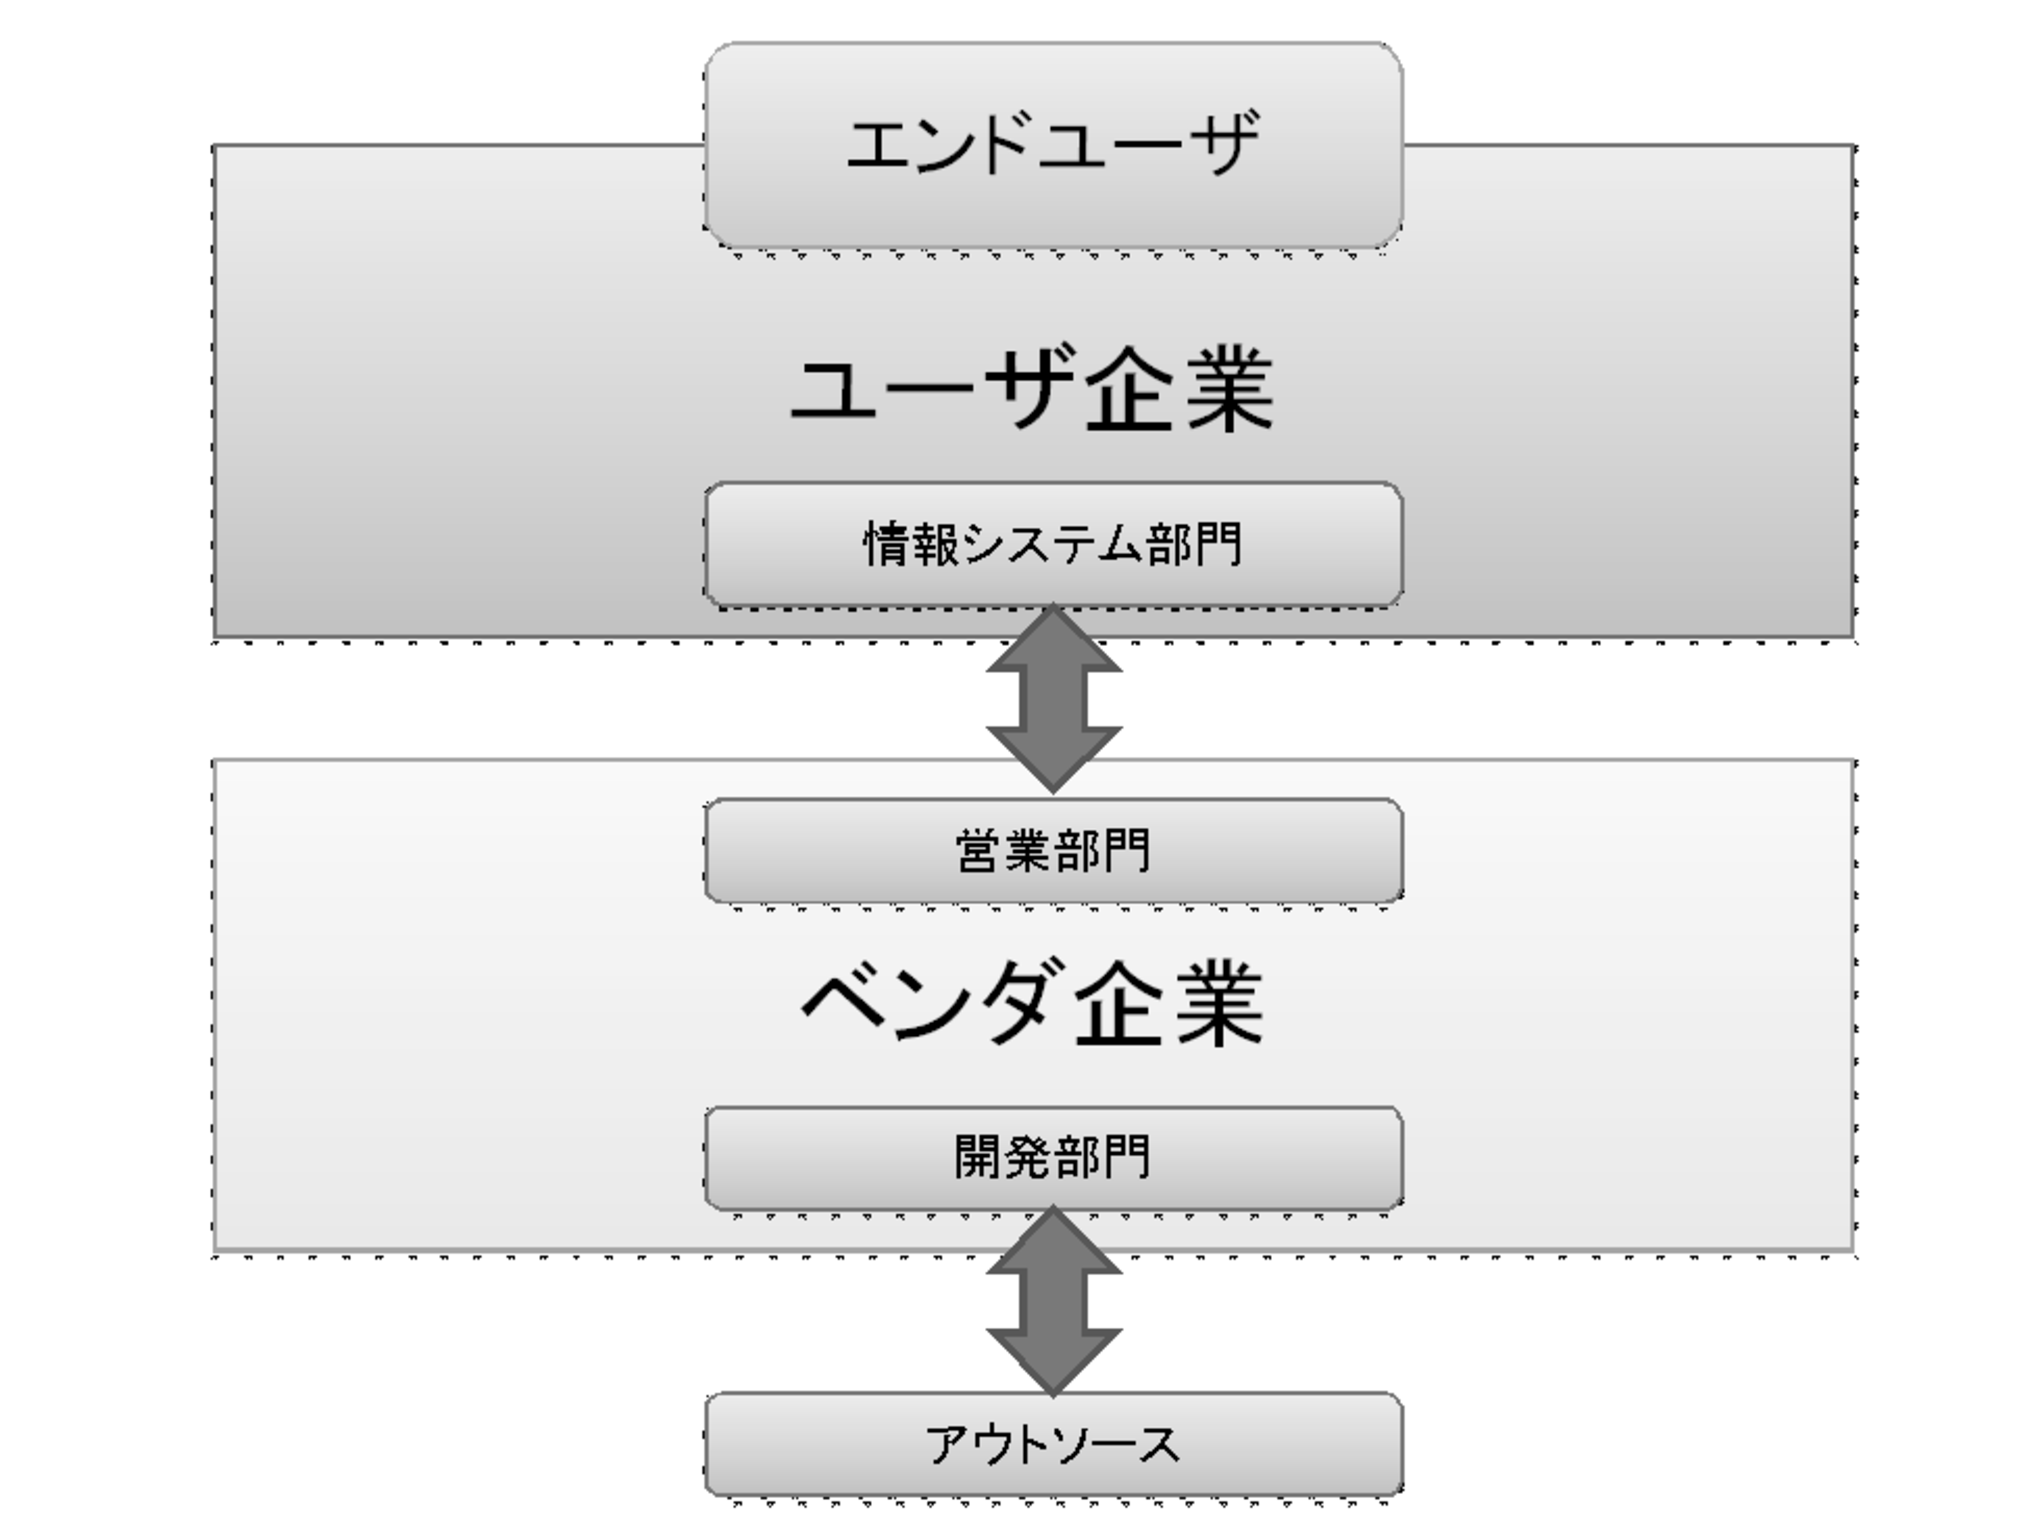
\includegraphics[width=6.5cm]{figs/user_vendor_model.eps}
		         \caption{ユーザ企業とベンダ企業の構造}
		         \label{fig:user_vendor_model}
	         \end{center}
         \end{wrapfigure}
	
	\begin{flushleft}
		■IT産業界の現状における構造的な問題
	\end{flushleft}

    前項の目的を設定した背景には,{\bf 我が国におけるソフトウェア産業界の構造上の問題}がある.
	一般的なソフトウェア開発ビジネスにおいては    
    ITを提供するベンダ企業と,自社のサービスのためにITを利用するユーザ企業との間には
    明確な対立構造が存在する.
    このため,
    両者のコンフリクトをマネジメントすることがソフトウェア開発チームに求められ,
    {\bf コ・クリエイティブにソフトウェアを開発することが非常に難しい}.
    
    図\ref{fig:user_vendor_model}は,従来のソフトウェア開発における
    ユーザ企業とベンダ企業との関係構造を模式化したものである.
    本来,ベンダ企業にとっては実際にソフトウェアを利用するエンドユーザに有益なプロダクトを製造する
    ことが最大のミッションであるはずだ.
    ところが,エンドユーザとベンダ企業の開発部門やアウトソース先企業との間には
    図に示した通り,幾重にも壁が存在している.このため,
    {\bf エンドユーザが求めるソフトウェアを正しく製造することは構造的に困難}である.
    
    % 一番上に示した「エンドユーザ」とは,実際にソフトウェアを利用するユーザ(個人)である.エンドユーザは「ユーザ企業」に所属し,
    % 企業が提供するサービスを実現するために情報システムを利用する.近年は,B2C型でサービスを提供する企業が増えたことから,
    % エンドユーザはユーザ企業の外部に存在し,Web等でユーザ企業が提供するサービスを利用する場合も見られる.
    
    % このようなソフトウェア開発を行う場合,一般的にユーザ企業にある「情報システム部門」がシステム開発を主導することになる.
    % 情報システム部門は複数の「ベンダ企業」に対してRFP(Request For Proposal)を提示し,これを受けてベンダが作成した
    % 提案を精査し,ソフトウェア開発を発注するベンダ企業を選定する.この一連のプロセスはベンダ企業の「営業部門」が担当する.
    
    % 営業部門が契約を取り付けた後,ベンダ企業の「開発部門」が実際のソフトウェア開発プロジェクトを開始することになる.
    % このとき,ベンダ企業内で必要なリソースが調達できない場合,ベンダ企業は社外の企業等に対して「アウトソース」を行う.
    % いわゆる下請けの関係であり,近年は人件費の安い海外にアウトソースすることも多い.
    
	% \begin{flushleft}
	%	■IT産業の構造変化
	% \end{flushleft}

    翻って世界に目を向けると,以上述べてきた{\bf ユーザ企業とベンダ企業が対立する構造に依らない,
    新しいタイプのソフトウェア開発企業が登場}してきている.例えば,
    GoogleやFacebookなどの有力な企業は,自らの顧客であるユーザとインタネットを通じて
    直接的にコミュニケーションをしながら,
    自社のプロダクトをグローバルに提供することでビジネス的な成功を収めている.
    
    更に,App StoreやGoogle Playといったスマートフォン向けアプリの
    マーケットが登場しており,個人であっても直接ソフトウェアプロダクトをマーケットに投入することさえ容易になってきたことも,
    現在のソフトウェア産業における大きな構造変化である.
    
         \begin{wrapfigure}[11]{r}{6.5cm}
			\vspace{-2cm}
         	\begin{center}
		         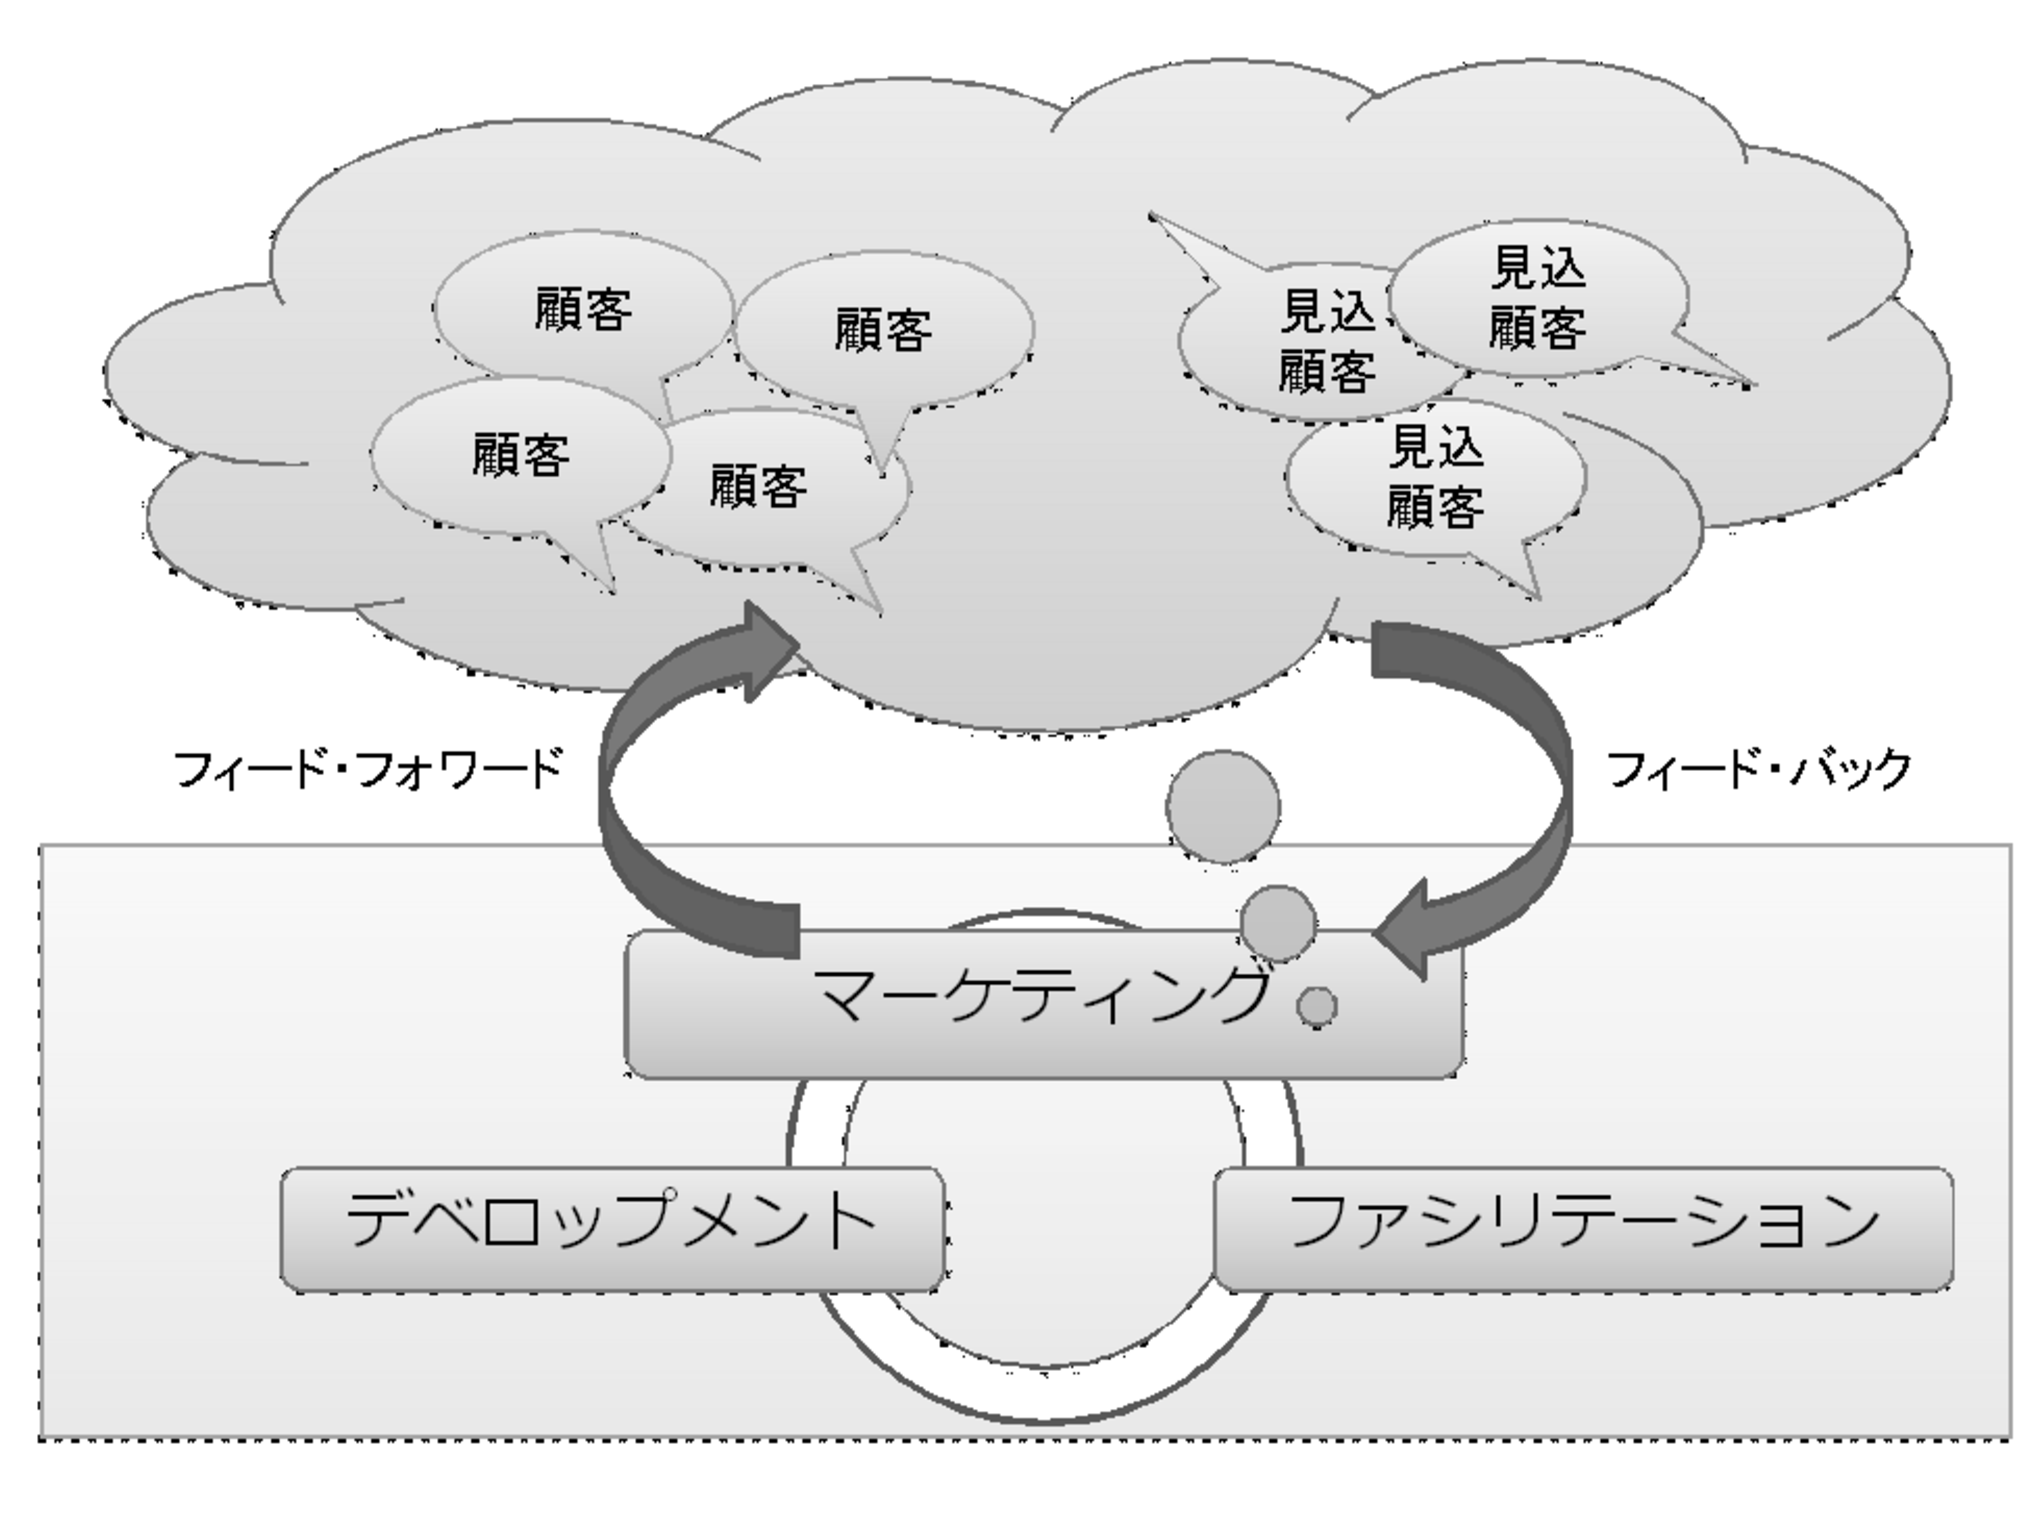
\includegraphics[width=6.5cm]{figs/CcSD.eps}
		         \caption{コ・クリエイティブなソフトウェア開発チームの振る舞い}
		         \label{fig:CcSD}
	         \end{center}
         \end{wrapfigure}
    
	\begin{flushleft}
		■次世代のソフトウェア開発者チームの育成
	\end{flushleft}

    ここまでの分析から,今後は{\bf 従来型の「ユーザ・ベンダ型モデル」は急速に存在感を失い,新しいタイプの企業が成長してくる}ものと予測する.
    本研究者はその際の中核概念が「コ・クリエイション」であると考える.
    
    すなわち,
    適時的にプロダクトをマーケットへ投入することで得られるマーケットからの``フィード・バック''や,
    将来的なマーケットの動向を予測して前もって製品に反映させる``フィード・フォワード''
    など,マーケットとの対話を通してプロダクトを生み出しうるソフトウェア企業が求められる.
    これは,マーケットとのコ・クリエーションのプロセスであり,
    その構造は図\ref{fig:CcSD}で示される.
    % 図\ref{fig:user_vendor_model}で示したモデルと比較すると,
    % 開発チームが直接マーケットとの対話を行う点で大きく異る.
    加えて,今後はグローバルなマーケットに対してのプロダクト開発も視野にいれておく必要があり,
    このような環境で迅速にソフトウェア開発ができる能力を備えた人材育成が望まれる.
    
    そこで,本研究ではこの
    {\bf 「コ・クリエイティブ型ソフトウェア開発」に対応できる知識や技術を持った人材を育成するための
    新しい教材と教授法について研究開発}することを目的とする.
    近年,ソフトウェアの開発プロセスを教育するためのメソッドとして,
    PBLが効果を上げている\KLcite{pub:matsuzawa-2008}.
    ただし,既存のPBLではユーザ・ベンダ型の構造を前提とした上で,プロジェクトの中で
    それぞれのロールを体験することによる教育効果を狙ったものが多い.
    これでは産業構造の変化を踏まえた次世代の開発者を育成する内容として不十分である.
    特に,{\bf グローバルなマーケットとのコ・クリエイティブな対話}のプロセスや,そのベースとなる迅速なソフトウェア開発のための
    {\bf チームとしてのアジャイル性を獲得する方法の体得}を柱に再構成する必要があろう.
    
    以上の背景を踏まえ,次世代のソフトウェア開発者を育成するための
    {\bf 「コ・クリエイティブなソフトウェア開発者を育成するPBL型教育」の手法を確立}し,必要な教材やWebサービスとともにパッケージ化し,
    {\bf 様々な教育機関における教育に提供}できる成果を得ることを本研究の目的とする.
    
	\vspace{1cm}
	\begin{thebibliography}{99}
		\bibitem{wired} 顧客とのco-creationプラットフォーム-ベストプラクティ, \\
                        \tt{http://wired.jp/2011/09/29/},  2012-10-24参照
        \bibitem{oss} クリス・ディボナ他, オープンソースソフトウェア―彼らはいかにしてビジネススタンダードになったのか,
        				オライリー・ジャパン, 1999-07
	\end{thebibliography}
%end  研究目的 ====================
}

%====================================
%form: kiban_c_form_03-04.tex ; user: kiban_c_03-04_plan.tex
%========== S-1-8 基盤研究(C)(一般) =========
%===== p. 03-04 研究計画・方法 =============
\section{研究計画・方法}
%watermark: w08_plan_C
\newcommand{\研究計画と方法概要}{%
%begin  研究計画と方法概要===================
	本研究では実施期間内においてアジャイル(迅速)に教材の開発と適用を繰り返し,より教育効果の高い
	PBL用電子教材を作成する.
	これには,迅速な電子教材開発のための「アジャイル教材製作スタジオ」を構築し,
	コンテンツとして用いる動画や音声を素早く製作できるように工夫する.
	製作した電子教材は,学生や教員がPBL実施時にオン・デマンドで参照できるようにし,
	学生の自発的な学びを支援する.

	初年度はScrum型の開発プロセスの教材を作成し,以降,コ・クリエイティブなソフトウェア開発のために
	必要な内容を拡充させる.成果物は本学および他大学でのPBLにおいて複数回利用し,改善を繰り返す.
	また,電子教材はクラウド型のサービスを用いて利用者に
	広く提供するものとする.
%end  研究計画と方法概要 ====================
}

\newcommand{\研究計画}{%
%begin  研究計画===================
	
	% 半年ごとにサイクルを回す.リーンスタートアップを実施する.

         \begin{wrapfigure}[13]{r}{7.8cm}
     		\vspace{-1cm}
         	\begin{center}
		         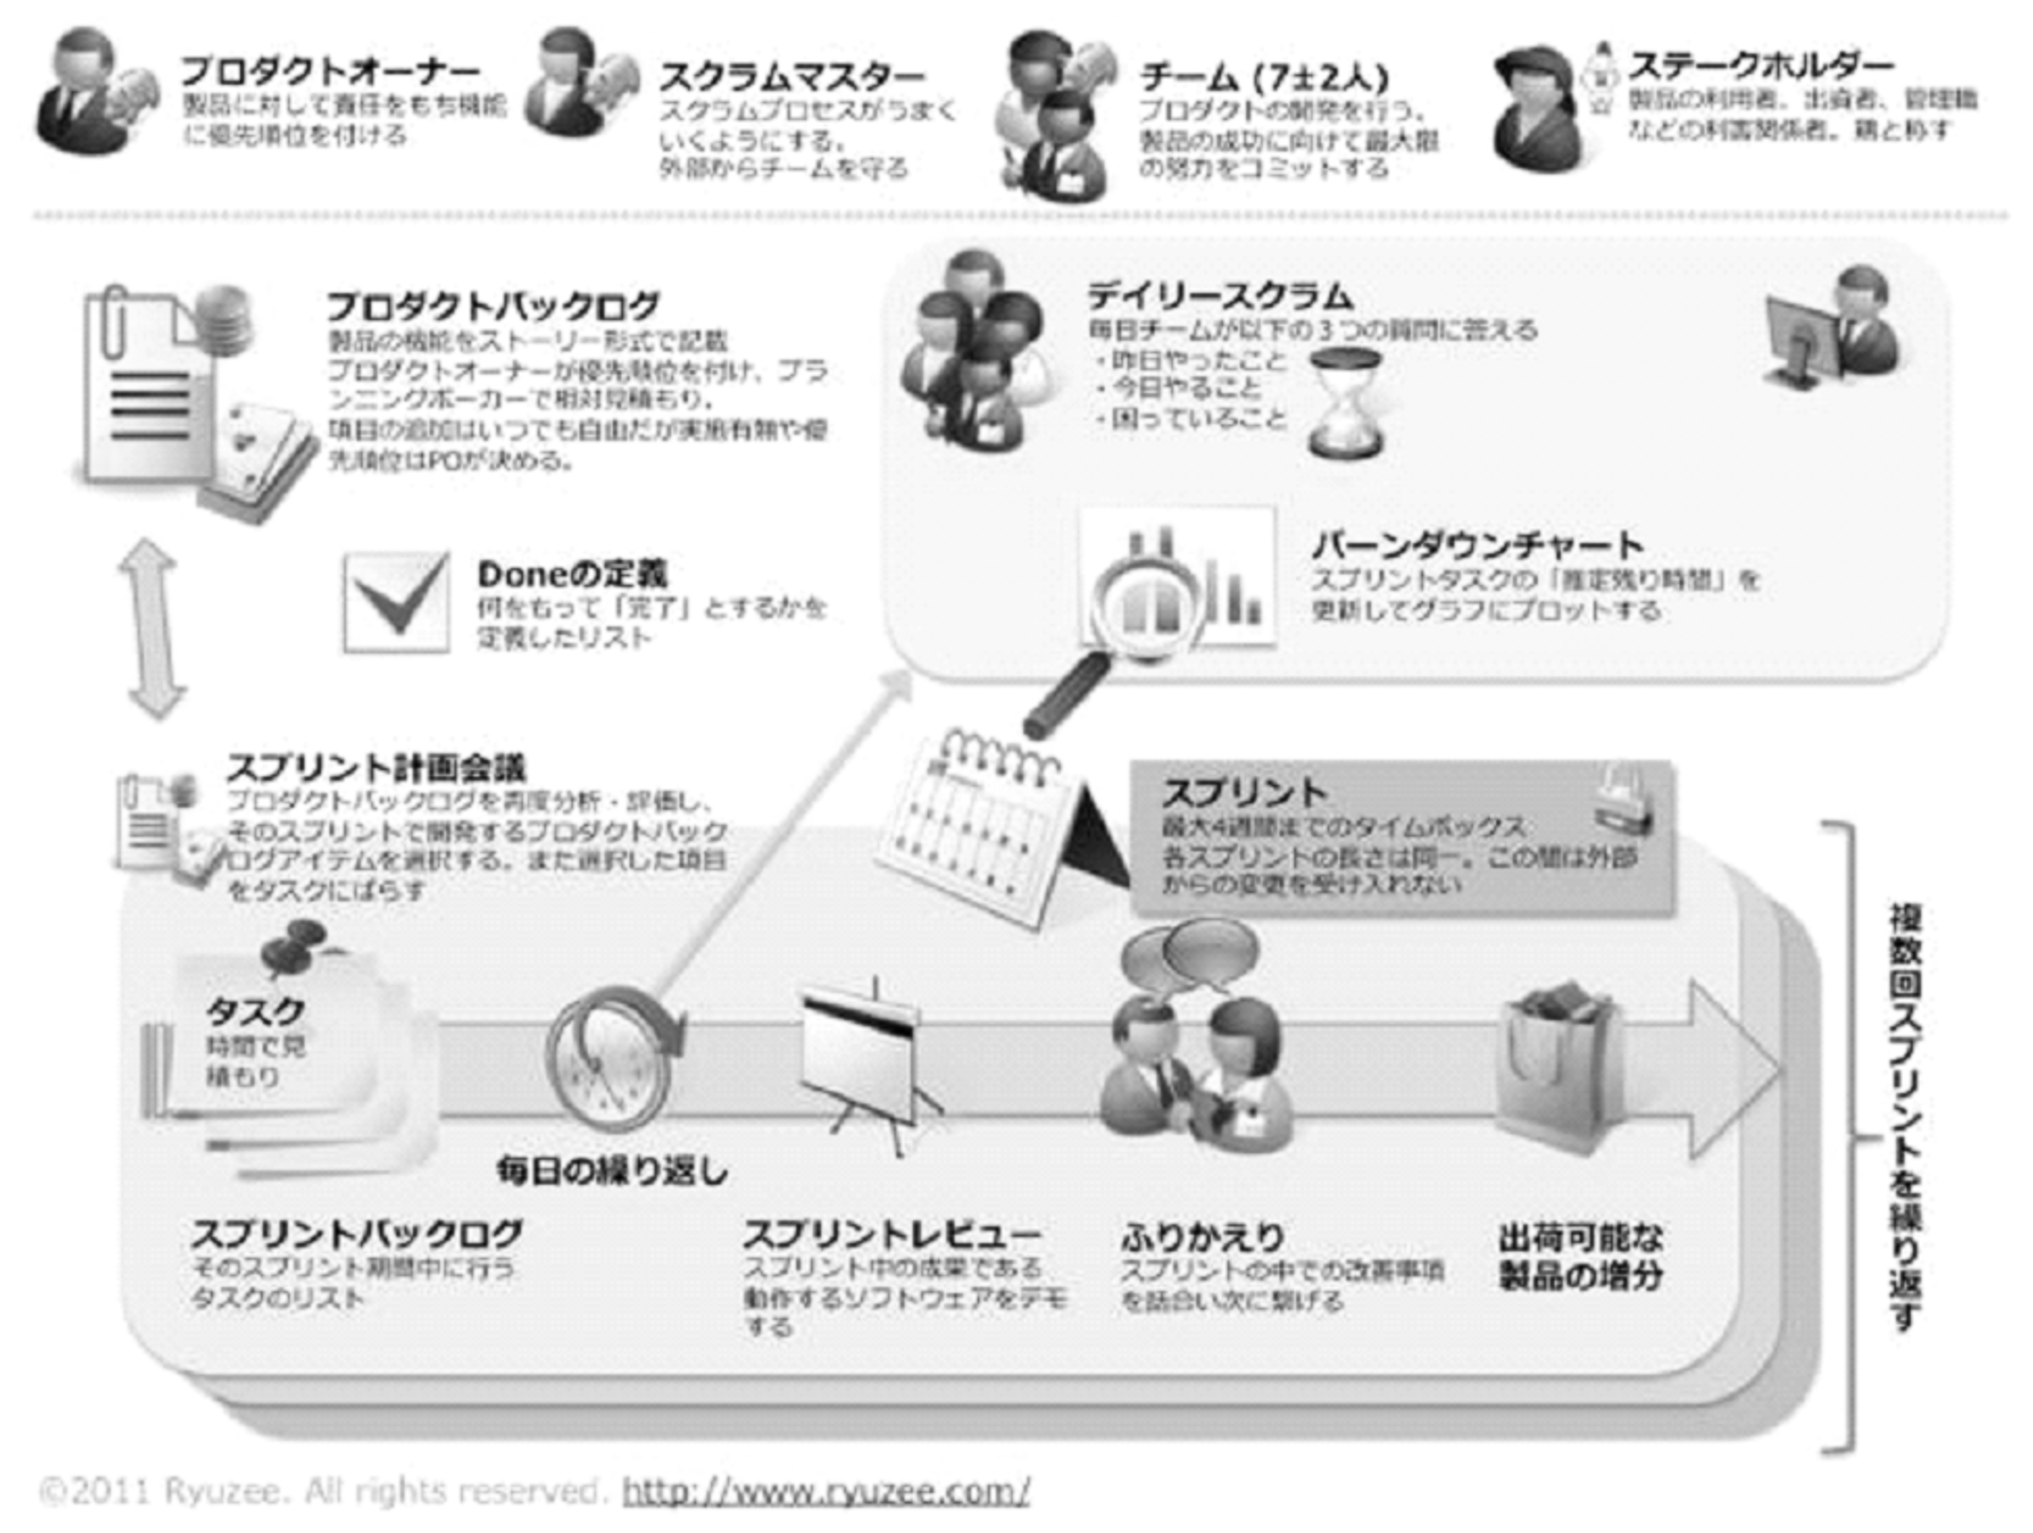
\includegraphics[width=7.8cm]{figs/scrum.eps}
		         \caption{Scrumの全体像(吉羽氏資料より)}
		         \label{fig:scrum}
	         \end{center}
         \end{wrapfigure}

	\begin{flushleft}
		■平成25年度の計画
	\end{flushleft}
	
	アジャイルなソフトウェア開発プロセスとして近年注目されているScrumは,
	野中らが日本企業のベストプラクティスについて述べた文献\cite{nonaka}が起源だとされる.
	これをSutherlandらが1990年代半ばにソフトウェア開発プロセスとして定義した.
	{\bf Scrum は他のソフトウェア開発方式と比べて非常にシンプル}であり,
	その全体像は図\ref{fig:scrum}でほぼ網羅されている.このため
	学習すべき知識項目の数はさほど多くない.その反面,
	{\bf 実際にScrumをプロジェクトで実施できるようになるには相当の訓練が必要}である.

	このようなスキルの獲得のためにはScrum型でプロジェクトを行うPBLを実施することにより,高い教育効果が見込める.
	しかしながら,大学の教室で学生がScrumを学ぶことに適した既存の教材は見当たらない.また,指導する教員にとっても
	Scrumの概念を深く理解して学生を指導することは難しい.

	よって,研究初年度は{\bf Scrum型のプロセスを学習するためのPBL用教材を製作}
	することを目標とする.そのためのアプローチとして,Scrumを参考にしたアジャイルなプロセスを本研究の計画そのものにも取り入れ,
	{\bf アジャイルを学ぶ教材をアジャイルで製作する}という,ある種メタ的な手法をとる.
	研究自体をアジャイルで実施することの意義は,迅速に教材を作成し,授業を展開して効果を確かめ,さらなる改善を行うというプロセスを
	繰り返すことで,{\bf 教材の質を漸進的に向上}できることにある.
	
	{\bf Scrumはチームによる自己組織化や,作業プロセスの改善
	などを重視するのが特徴}である.
	これらは,実際にプロジェクトを行なってみて
	具体的な課題に直面してみないとその重要性に気づかないことが多い.
	そこで本研究で開発するScrum教育のための教材は,
	{\bf PBLを実施中の学生および教員がオンデマンドでアクセス}できる
	ようにする.
	これにより,学生がプロジェクトを実施中に具体的な課題に気づき,その解決を自主的に求めることを支援できるようになる.
	
	前述のとおり,
	本研究は研究自体もアジャイルで行うことため,迅速に教材を制作し,実際に教育の現場に教材を提供してフィードバックを得,
	必要な内容で漏れていることがあれば追加したり,わかりにくい箇所を改善させたりといった,反復型のプロセスにより
	内容を充実させていくことを基本的な計画とする.
	
	その最初のステップとしては,図\ref{fig:scrum}に基づき,Scrumの全体概要,
	役割分担(Scrum MasterやProduct Owner,Team Memberなど),
	成果物(プロダクトバックログ,スプリントバックログ,バーンダウンチャートなど),
	プロセス(スプリント計画会議,デイリースクラム,振り返りなど)に関する教材を用意しておく.
	加えて,Scrumで実際にソフトウェア開発を行うときに利用するクラウド型のツールについても解説する.

         \begin{wrapfigure}[11]{r}{6cm}
			\vspace{-1cm}
         	\begin{center}
		         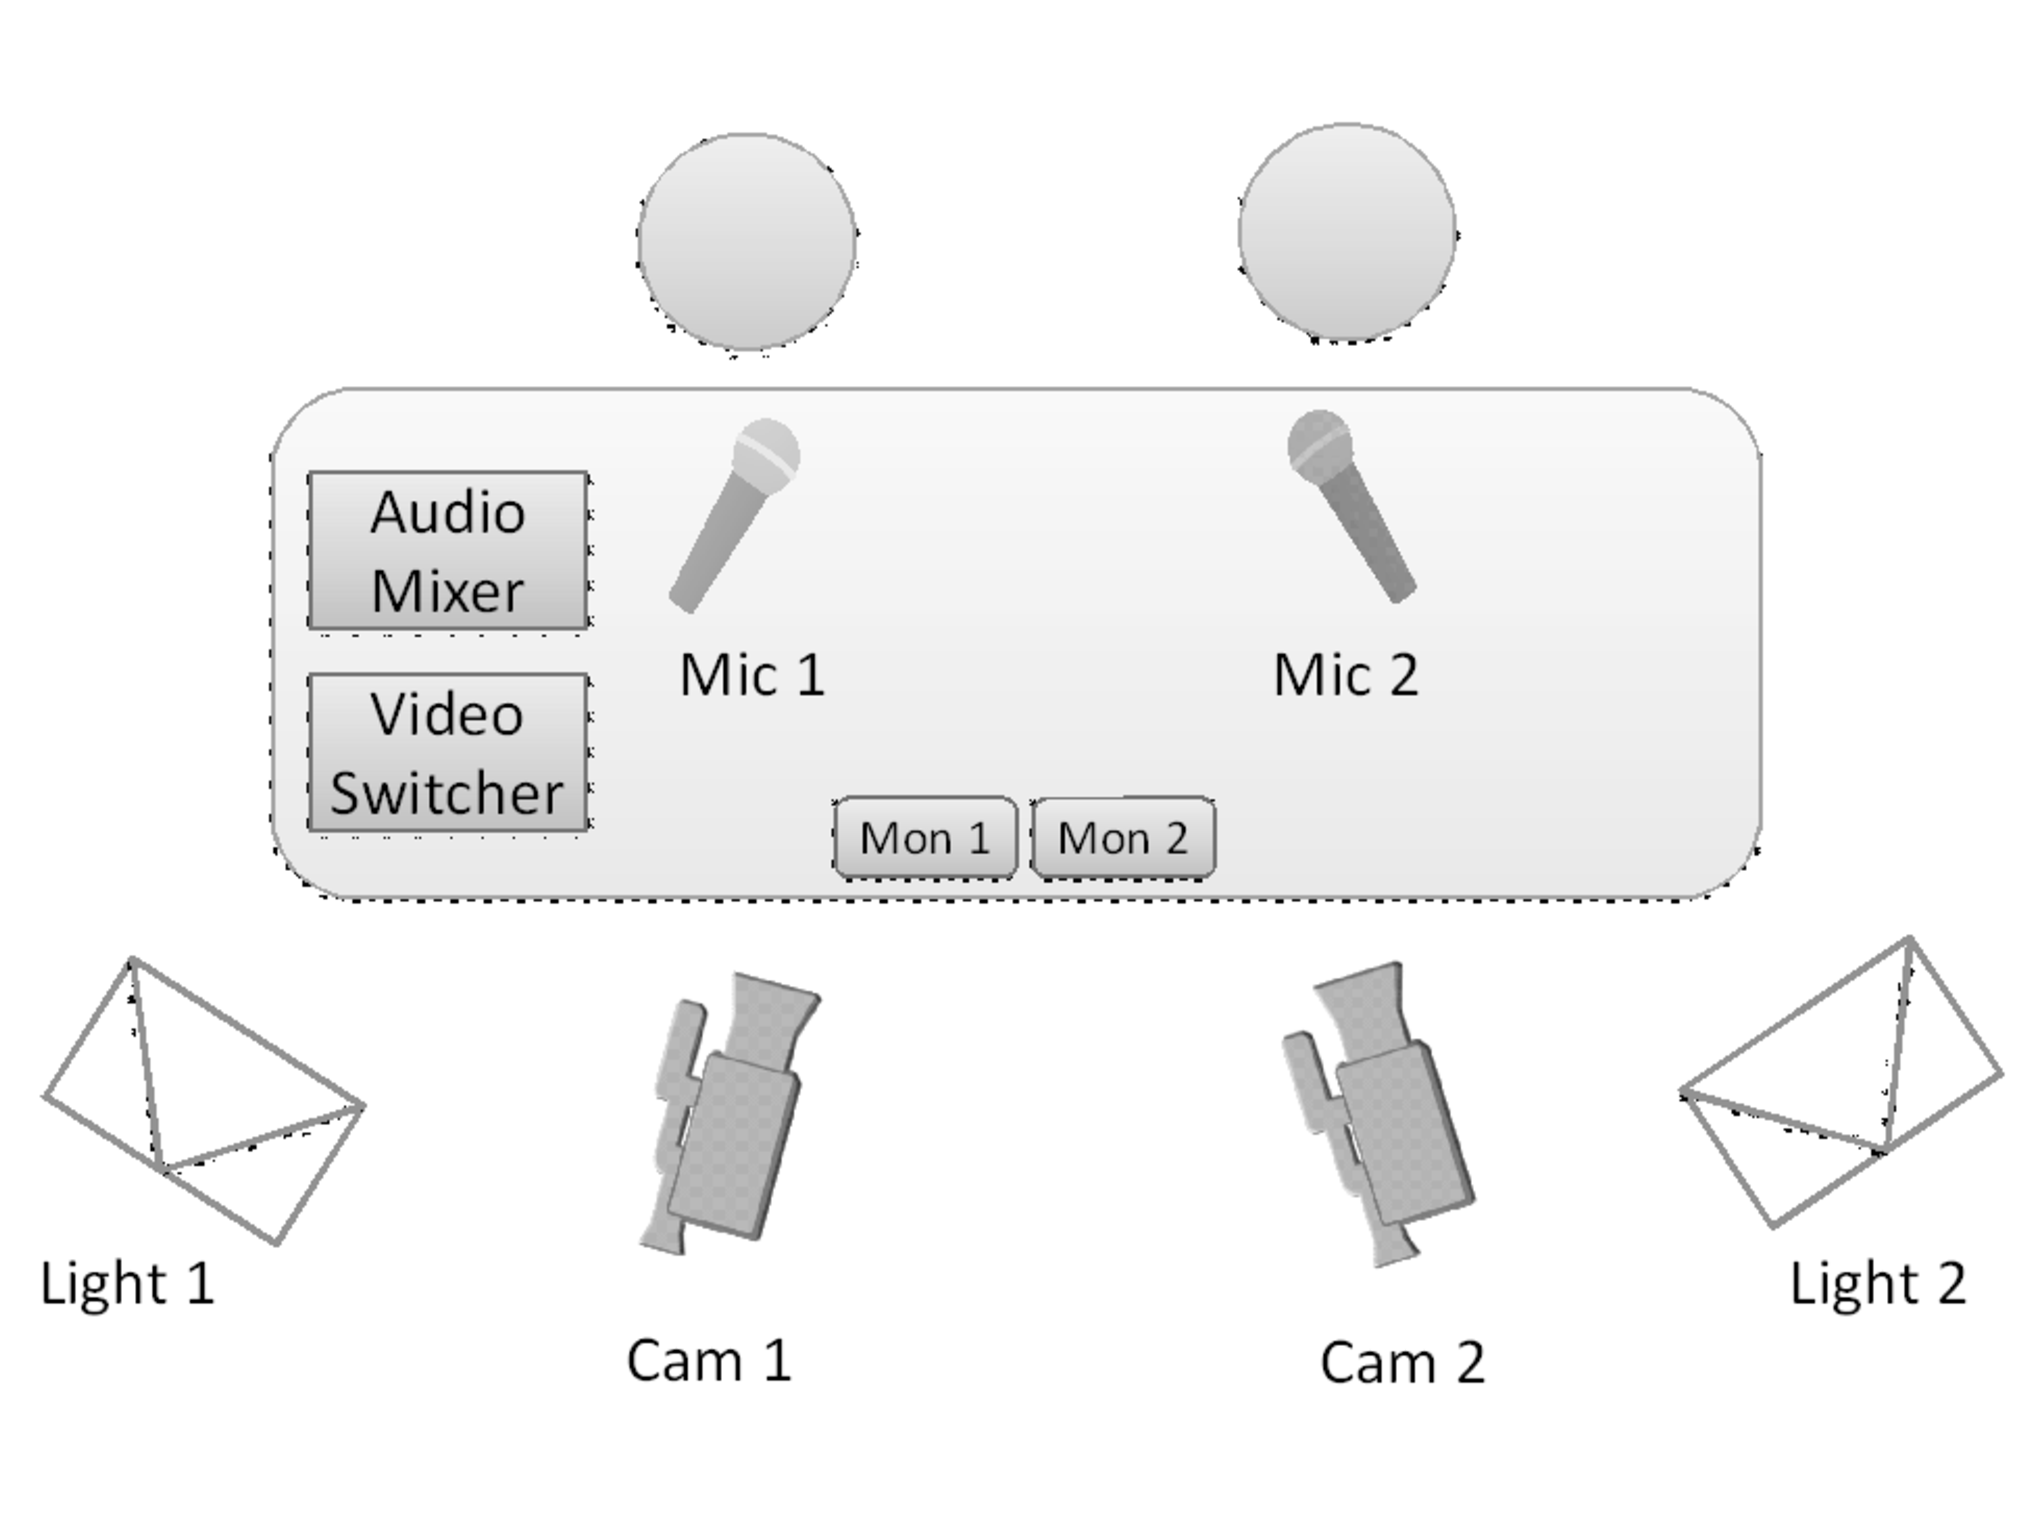
\includegraphics[width=6cm]{figs/studio.eps}
		         \caption{アジャイル教材制作スタジオ}
		         \label{fig:studio}
	         \end{center}
         \end{wrapfigure}

	また,ゲーム感覚で取り組めるアンプラグドなワークショップを
	体験させるのもScrumの学習において効果的である.そこで,この教材では各種のワークショップ(紙飛行機作成,ボール渡し,
	Manager-Workerゲームなど多数)を紹介し,実施するための方法についても内容に含める.

	以上の研究計画を遂行する上での課題となるのは,音声や映像を伴う高クォリティの電子教材の製作に要する手間の低減である.
	そこで本研究では,
	業務でプロが使用するレベルの音響・映像機器(図\ref{fig:studio})と,
	様々な編集に必要となるコンピュータをセットにした{\bf 「アジャイル教材製作スタジオ」の構築}を研究テーマの1つとする.
	このスタジオにより迅速な電子教材製作を可能とすることを目指す.

	なお,本教材の研究開発全般において,Scrumコーチの認定資格を有する専門家に依頼し,内容等についてレビューして頂く.

	\begin{flushleft}
		■平成26年度以降の計画
	\end{flushleft}
	
	2年目からは,{\bf Scrumをベースとしたコ・クリエイティブ・ソフトウェア開発プロセスを学ぶための教材}
	を順次,追加する.

	クラウド技術などの発展により,開発したプロダクトをインターネット上にあるグローバルなマーケットに投入することが
	容易になってきている.学生が実施するPBLの成果物を現実のマーケットで公開し,
	その評価を得ることも難しくなくなった.
	
	そこで,
	{\bf PBLでの成果物を実際にマーケットに投入し,コ・クリエイティブにソフトウェアの製品価値を高める体験をするための教育コンテンツ}を追加する.
	加えて,各種のSocial Networkなどを利用して
	{\bf グローバルなコミュニケーションを通したコ・クリエイティブなソフトウェア開発}を行えるようにする教材開発にも取り組む予定である.

	本研究で得た知見は,本学におけるPBL型授業や,他大学(静岡大学・慶應大学等)の授業に随時導入し,その結果を積極的に発表する.
	発表する媒体としては,関連する学会等のほか,SNSやブログでも情報提供を行なっていく.
	これにより,{\bf 本研究における成果を広く社会に還元}するものとする.
	
	また,将来的には,作成した電子教材を各国語(英語,中国語・韓国語及びASEAN諸国の言語など)に翻訳し,
	海外の技術者と日本の学生とが共同で取り組むことのできるグローバルなPBLへと展開したい.
	
	\vspace{1cm}
	\begin{thebibliography}{99}
		\bibitem{nonaka} H.~Takeuchi, I.~Nonaka: The New New Product Development Game, Harvard Business Review January-February, 1986
		% \bibitem{lean-startup} エリック・リース: リーン・スタートアップ ―ムダのない起業プロセスでイノベーションを生みだす, 日経BP社, 2012
	\end{thebibliography}
%end  研究計画 ====================
}

%form: kiban_c_form_05.tex ; user: kiban_c_05_preparation_final_year.tex
%========== S-1-8 基盤研究(C)(一般) =========
%===== p. 05 準備状況等、最終年度の応募 =============
\section{準備状況等、最終年度の応募}
\subsection{準備状況等}
\newcommand{\準備状況等}{%
%begin  準備状況等 ===================
	\underline{本研究を実施するための研究施設}としては,
	産業技術大学院大学(AIIT)では2006年度より情報システムのアーキテクトを育成するための
	PBLを実施しており\KLcite{pub:tozawa-pbl-2009},本研究はこの一環として施設等を利用できる.
	また,このPBLにおいて,本研究者らはソフトウェア開発方法論を教育する目的で,
	アジャイル型開発プロセスを
	指導した実績を有し,ここから得られた知見も活用する.
	特に,2009年度以降は,ベトナム国家大学の学生と共にグローバルPBLを展開し,
	海外の技術者との共同プロジェクトを実施して,その成果を発表している
	\KLcite{pub:kizaki-global-2011b}\KLcite{pub:kizaki-global-2011c}\KLcite{pub:kizaki-global-2011a}%
	\KLcite{pub:chubachi-global-2010}%
	\KLcite{pub:tozawa-global-2009}
	.
	加えて,慶應大学で開講している「協創型ソフトウェア開発」の授業では2011年度から
	アジャイル型ソフトウェア開発手法であるScrumを全面的に導入し,コ・クリエイティブなソフトウェア開発者教育の試行を始めている.
	
	\underline{研究分担者}の役割は,製作する教材の構成や内容について分担し,
	この教材を用いたPBLの指導も行い,改善点を抽出する.また,学会等を通した研究成果の公開も共同で行う.
	
	\underline{本研究の研究成果を発信}するためには,AIITにおけるPBL全体を支援する情報インフラストラクチャに関する研究の知見
	\KLcite{pub:chubachi-ipbl-2012}\KLcite{pub:chubachi-ipbl-2011}%
	\KLcite{pub:chubachi-ipbl-2009b}\KLcite{pub:chubachi-ipbl-2009a}
	を活用し,クラウド型のサービスを提供する.
%end  準備状況等 ====================
}

\subsection{研究計画最終年度の応募}
\newcommand{\研究計画最終年度の応募の研究種目名}{%
%begin  研究種目名 ===================
%end  研究種目名 ====================
}

\newcommand{\研究計画最終年度の応募の審査区分}{%
%begin  審査区分 ===================
%end  審査区分 ====================
}

\newcommand{\研究計画最終年度の応募の課題番号}{%
%begin  課題番号 ===================
%end  課題番号 ====================
}

\newcommand{\研究計画最終年度の応募の研究課題名}{%
%begin  研究課題名 ===================
%end  研究課題名 ====================
}

%\KLTextBox{494}{423}{522}{369}{}{%
\newcommand{\研究計画最終年度の応募の研究期間初年度}{%
%begin  研究期間初年度 ===================
%end  研究期間初年度 ====================
}

\newcommand{\研究計画最終年度の応募の計画と成果}{%
%begin  特別推進研究又は基盤研究による研究計画及び研究成果 ===================
	該当なし
%end  特別推進研究又は基盤研究による研究計画及び研究成果 ====================
}

\newcommand{\研究計画最終年度の応募の理由}{%
%begin  研究計画最終年度前年度の応募をする理由 ===================
%end  研究計画最終年度前年度の応募をする理由 ====================
}

%====== end of page =====================================
%form: kiban_c_form_06-07.tex ; user: kiban_c_06-07_publications.tex
%========== S-1-8 基盤研究(C)(一般) =========
%===== p. 06-07 研究業績 =============
\section{研究業績}		
%watermark: w14_pub_C
% 2012-09-01 Taku
\newcommand{\年と名前と研究業績}{%
%begin  研究業績 ===================
		% 2013年度から始まった2カラムのtabularです。
%ーーーーーーーーーーーーーーーーーーーーーーーーーーーーーーーーーーーーーーーーーーーー
%		\KLcite{pub:theoegg} のようにして業績番号を文中に入れられます。
%ーーーーーーーーーーーーーーーーーーーーーーーーーーーーーーーーーーーーーーーーーーーー
	2012 {\small 以降} \\
		中鉢 欣秀
		& \KLbibitem \label{pub:chubachi-ipbl-2012} \me, 小山裕司: AIITにおけるプロジェクト型学修(PBL)のためのBacklogシステムの導入, 情報処理学会 第19回IOT・第39回EVA合同研究発表会, 島根県松江市, 2012-09-27.(査読無)\\ 
		& \KLbibitem \me, 小山 裕司, 石島 辰太郎: 産業技術大学院大学のICT環境の運用と課題, 研究報告インターネットと運用技術(IOT), 一般社団法人情報処理学会, Vol.2012-IOT-16, No.11, pp.1-4, 2012-03-08.(査読無) \\
		松澤 芳昭
		% & \KLbibitem 早川 勝,野沢 光太郎,\unedrline{松澤 芳昭},酒井 三四郎: "オブジェクト指向モデリング教育のためのオブジェクト図自動生成システムの設計と評価", 情報処理学会論文誌, Vol.54, No.1, 2013 (印刷中) (査読有) \\
		% & \KLbibitem 新野 朝丈, 平山 雅樹, \underline{松澤 芳昭}, 児玉 公信, 太田 剛: "ポータルサイト運営者のための軽量マッシュアップ開発ツールの提案と評価", 情報処理学会論文誌, Vol.54, No.1, 2013 (印刷中) (査読有) \\
		% & \KLbibitem \underline{Y.~Matsuzawa}, J.~Oshima, R.~Oshima, S.~Sakai: Learners' Use of SNA-based Discourse Analysis as a Self-Assessment Tool for Collaboration, International Journal of Organisational Design and Engineering, 2012,(印刷中)(査読有) \\
		& \KLbibitem 野口 靖浩, \underline{松澤 芳昭}, 森 孝夫,島 聰司,塩見 彰睦:合宿とPBLによる組込みシステムアーキテクト養成プログラムの設計と評価,日本教育工学会論文誌,Vol.36, No.1, pp.21-33, 2012. (査読有) \\
		& \KLbibitem 野口 靖浩, \underline{松澤 芳昭}, 島 聰司, 塩見 彰睦: 組込み人材育成研修後の上司による「行動変容」評価の実践とSCATによる分析, 工学教育, Vol.60, No.3, pp.86-91, 2012.05. (査読有) \\
	\hline%----------------------------------------------
	
	2011 \\
		中鉢 欣秀
		& \KLbibitem \label{pub:chubachi-ipbl-2011}\me, 小山 裕司: PBLを支援するコラボレーティブツールに関する考察, 産業技術大学院大学紀要, No.5,pp.100-108, 2011 (査読有)\\
		% & \KLbibitem 小山 裕司, \me: 外部アカウント認証を使った本人確認付き利用者認証の仕組み, 産業技術大学院大学紀要, No.5,pp.75-80, 2011(査読有) \\
		& \KLbibitem 小山 裕司, \me, 土屋 陽介: ソーシャルメディアを活用したコネクション構築支援, 情報処理学会研究報告. コンピュータと教育研究会報告, 一般社団法人情報処理学会, Vol.2011, No.3, pp.1-6, 2011-12-10.(査読無) \\
		& \KLbibitem 土屋 陽介, 小山 裕司, \me: 授業配信システムの設計と開発, 情報処理学会研究報告. コンピュータと教育研究会報告, 一般社団法人情報処理学会, Vol.2011, No.2, pp. 1-7, 2011-12-10.(査読無) \\
		& \KLbibitem \label{pub:kizaki-global-2011b} 木崎 悟, 成田 亮, 丸山 英通, 土屋 陽介, 成田 雅彦, \me: 国際PBLにおける的確な仕様の伝達とチケット駆動による開発作業の効率化, ソフトウェアエンジニアリングシンポジウム2011, 東京女子大学, 2011-09.(査読有) \\
		& \KLbibitem \label{pub:kizaki-global-2011c} 木崎 悟, 丸山 英通, 土屋 陽介, \me: ソフトウェア開発PBLへのチケット駆動開発の適用による共同作業の改善, プロジェクトマネジメント学会 2011年度秋季研究発表大会, 産業技術大学院大学, 2011-09.(査読無) \\
		% & \KLbibitem \me: 目的/手段展開に基づくソフトウェアアーキテクチャの仕様化, 要求工学WGワークショップ, 情報処理学会, 礼文島, 2011-06-24 \\
		& \KLbibitem \label{pub:kizaki-global-2011a} 木崎 悟, 成田 亮, 丸山 英通, \me: グローバルなソフトウェア開発におけるマネジメント手法, 情報処理学会 第172回ソフトウェア工学研究会, 早稲田大学, 2011-05-17.(査読無) \\
		% &  \KLbibitem 木崎 悟, 成田 亮, 丸山 英通, 土屋陽介, \me: タスク管理を支援するタスクコンシェルジュの開発, 電子情報通信学会総合大会ポスターセッション, 東京都市大学, 2011-03-16. \\
	\hline%----------------------------------------------
	2010 \\
		中鉢 欣秀
		&  \KLbibitem \label{pub:chubachi-global-2010} \me, 成田 雅彦, 戸沢 義夫: 加藤由花, 戸沢義夫: ベトナム国家大学とのグローバル PBL から得た知見, 産業技術大学院大学紀要, pp.1-4, 2010. (査読有) \\
		&  \KLbibitem \me: 遠隔会議システムを用いた国際PBLから得た知見, 日本e-Learning学会学術講演会論文誌, 東京都千代田区, 2010-11-14.(査読無) \\
		&  \KLbibitem \meen, Y.~Kato, Y.~Tozawa: Web-based groupware supporting PBL effectively, 1st Asia-Pacific Joint PBL Conference 2010, 2010-10-24(査読有) \\
		&  \KLbibitem \label{pub:nishino-2010} R.~Nishino, M.~Kojima, O.~Oka, T.~Okino, T.~Sugita, Y.~Tsuchiya, H.~Koyama, Y.~Tozawa, \meen: Experience Gained through International PBL in Software Development, 1st Asia-Pacific Joint PBL Conference 2010, 2010-10-23(査読有) \\
		% &  \KLbibitem 木崎 悟, 成田 亮, 丸山 英通, \me, 長尾 雄行: GTD初心者のタスク管理を支援するタスクコンシェルジュの開発, 第9回情報科学技術フォーラム, 福岡県福岡市, 2010-08-20 \\
		&  \KLbibitem \me, 小山 裕司, 石島 辰太郎: ICTを基盤とした高度専門職教育, 情報教育シンポジウム論文集, 情報処理学会, 情報処理学会シンポジウムシリーズ IPSJ Symposium Series Vol.2010, No.6, pp.133-138, 群馬県渋川市, 2010-08-19.(査読無) \\
		% &  \KLbibitem \me: ワークショップ実行委員長業務のSBVA法による要求分析, 要求工学ワーキンググループ ワークショップ, 情報処理学会, 礼文島, 2010-06-17 \\
		% &  \KLbibitem S.~Ishijima, H.~Koyama, \meen, F.~Harashima: ICT-based Learning System of AIIT for the professional education in Japan, 9th International Conference on Information Technology Based Higher Education and Training (ITHET 2010), 2010-04-29 \\
		松澤 芳昭
		& \KLbibitem \underline{Y.~Matsuzawa}, Y.~Noguchi, T.~Mori, S.~Shima, A.~Shiomi: ESAD: An Intensive Retreat Program for Embedded System Architect Developing, 17th APSEC, pp.90-97, 2010.(査読有) \\
		& \KLbibitem \underline{Y.~Matsuzawa}, J.~Oshima, R.~Oshima, Y.~Nihara, S.~Sakai: KBDeX: A Platform for Exploring Discourse in Collaborative Learning, Collaborative Innovation Networks(COINs) 2010. (Web出版) (査読有) \\
	\hline%----------------------------------------------

	2009 \\
		中鉢 欣秀
		&  \KLbibitem \label{pub:chubachi-ipbl-2009b} \me, 加藤由花, 戸沢義夫: PBL用情報インフラストラクチャの構築と運用, 産業技術大学院大学紀要, pp.109-116, 2009 (査読有) \\
		&  \KLbibitem \label{pub:tozawa-pbl-2009} Y.~Tozawa, Y.~Kato, \meen: Efforts to ensure the quality of PBL education in the graduate school of Information Technology, Proceedings of the 2nd International Research Symposium on PBL, 3-4 December 2009, Melbourne, Australia, pp.1-9(査読有) \\
		% &  \KLbibitem \me: 要求分析モデリング支援システムの開発~SBVAエディタ~, 要求工学ワーキンググループ ワークショップ, 情報処理学会, 天橋立, 2009-10-22 \\
		&  \KLbibitem \label{pub:tozawa-global-2009} 戸沢 義夫, 成田 雅彦, \me, 土屋 陽介: Global PBL Feasibility Studyの実践と得られた知見, 情報処理学会 情報教育シンポジウム論文集, pp.167-174,2009-08-20.(査読無) \\
		% &  \KLbibitem \label{pub:ohrui-global-2009} 大類 優子,成田 雅彦,\me,土屋 陽介,戸沢 義夫: Global PBL Feasibility Studyの実践検証, 情報科学技術フォーラム講演論文集, FIT(電子情報通信学会・情報処理学会)推進委員会, 2009-08-20, Vol.8, No.4, pp. 515-516 \\
		&  \KLbibitem \label{pub:chubachi-ipbl-2009a} \me, 土屋 陽介, 長尾 雄行, 加藤 由花, 酒森 潔, 戸沢 義夫: グループウェア導入によるPBLの見える化, 日本e-Learning学会論文誌, Vol.9, pp.129-135, 2009-05.(査読有) \\
		% &  \KLbibitem \me: 要求記述演習によるロジカルシンキング教育の評価, 要求工学ワーキンググループ ワークショップ, 情報処理学会, 銚子, 2009-05-29 \\
        % &  \KLbibitem \me: 要求分析者育成のためのコミュニケーション能力教育, ウィンターワークショップ2009・イン・宮崎論文集, 情報処理学会, Vol.2009, No.3, pp.45-46, 宮崎, 2009-01-23 \\
		% &  \KLbibitem \me: 要求工学セッションの紹介~WW2010~, ウィンターワークショップ2010イン・倉敷論文集,情報処理学会,情報処理学会シンポジウムシリーズ IPSJ Symposium Series Vol.2010,No.3, pp.31-32, 2010-01-21 \\
		松澤 芳昭
		& \KLbibitem \underline{Y.~Matsuzawa}, A.~Shiomi, T.~Haraikawa, S.~Sakai: Two Challenges to Promote EVM on PBL in Software Engineering Education, 2nd International Research Symposium on PBL (IRSPBL'09), pp.1-10, 2009.(査読有) \\
		& \KLbibitem \underline{松澤 芳昭},大岩 元: 情報系学生を対象としたオブジェクト指向までのプログラミング入門教育の実践と課題, 情報教育シンポジウム(SSS2009),pp199-206, 2009.(査読有) \\
	\hline%----------------------------------------------

	2008 \\
		中鉢 欣秀
		% &  \KLbibitem 長尾 雄行, 土屋 陽介, 森本 祥一, \me: JavaScriptと非同期HTTPリクエストによる共同作業支援ミドルウェアの構築, 産業技術大学院大学紀要, Vol.2, pp.165-174, 2008(査読有) \\
		% &  \KLbibitem 森本 祥一, \me: シナリオの図解化による業務フロー分析, 産業技術大学院大学紀要, Vol.2, pp.193-208, 2008(査読有) \\
		&  \KLbibitem \me, 土屋 陽介, 長尾 雄行, 加藤 由花, 酒森 潔, 戸沢 義夫, PBLを見える化する協調作業支援環境の構築, 日本e-Learning学会2008年秋季学術講演会論文集, pp.72-79, 京都, 2008-11.(査読無) ※優秀賞受賞 \\
		% &  \KLbibitem \me, システム開発における仮説検証型の要求分析プロセス, 要求工学ワーキンググループ ワークショップ, 情報処理学会, 雲仙, 2008-10-23 \\
		% &  \KLbibitem 長尾 雄行, 土屋 陽介, 森本 祥一, \me: JavaScriptと非同期HTTPリクエストによる共同作業支援ミドウェアの構築, 情報処理学会論文誌:プログラミング, Vol.1, No. 1, pp.63-64, 2008-06 \\
		% &  \KLbibitem \me, 専門職大学院におけるモデリング教育とSBVA法, 要求工学ワーキンググループ ワークショップ, 情報処理学会, 奄美大島, 2008-05-15 \\
		% &  \KLbibitem 橋山 牧人,中鉢 欣秀, 大岩 元: 携帯ゲームアプリケーション開発を支援するオブジェクト指向を用いたフレームワークの開発, 情報処理学会第71会全国大会, pp.4-733-734,草津(滋賀), 2009年3月 (NII)
		松澤 芳昭
		% & \KLbibitem 杉浦 学,\underline{松澤 芳昭},岡田 健,大岩 元: アルゴリズム構築能力育成の導入教育:実作業による概念理解に基づくアルゴリズム構築体験とその効果,情報処理学会論文誌,Vol.49,No.10,pp.3409-3427, 2008(査読有) \\
		% & \KLbibitem 荒木 恵, \underline{松澤 芳昭},杉浦 学,大岩 元: プログラミング教育への導入のための情報システム概念に基づくアンプラグドワークショップ,情報教育シンポジウム(SSS2006),pp.163-170, 2008(査読有) \\
		& \KLbibitem \label{pub:matsuzawa-2008} \underline{松澤 芳昭},杉浦 学,大岩 元: 産学協同のPBLにおける顧客と開発者の協創環境の構築と人材育成効果, 情報処理学会論文誌,  Vol.49, No.2, pp.944-957, 2008(査読有) \\
%end  研究業績  ====================
}

\newcommand{\連携研究者の研究業績}{%
%begin  連携研究者の研究業績 ===================
		% 2カラムのtabularです。
%ーーーーーーーーーーーーーーーーーーーーーーーーーーーーーーーーーーーーーーーーーーーー
%		\KLciteB{pub:theoegg} のようにして業績番号を文中に入れられます。
%ーーーーーーーーーーーーーーーーーーーーーーーーーーーーーーーーーーーーーーーーーーーー
%end  連携研究者の研究業績  ====================
}

%===========================================================
 %=======================================================
%form: kiban_c_form_08.tex ; user: kiban_c_08_past_funds.tex
%========== S-1-8 基盤研究(C)(一般) =========
%===== p. 08 これまでに受けた研究費とその成果等 =============
\section{これまでに受けた研究費とその成果等}
\newcommand{\これまでに受けた研究費とその成果等}{%
%begin  これまでに受けた研究費とその成果等 ===================
	\begin{itemize}
		\item 科学研究費補助金 若手研究(B) ,2008~2009年度,
		    「情報システムアーキテクト育成のための遠隔教育システム」,研究代表者,3,900千円\\
		    本研究では社会人教育における利用を想定したモデリング遠隔教育支援シス
            テムを研究開発した.これを用いて,特にユーザ企業の社会人を対象としたモデリング
            教育支援環境を構築し,その有用性を確かめることができた.
    \end{itemize}
%end  これまでに受けた研究費とその成果等 ====================
}

%====== end of page =====================================
%form: kiban_c_form_09.tex ; user: kiban_c_09_relation.tex
%========== S-1-8 基盤研究(C)(一般) =========
%===== p. 09 研究計画と研究進捗評価を受けた研究課題の関連性 =============
\section{研究計画と研究進捗評価を受けた研究課題の関連性}
\newcommand{\研究計画と研究進捗評価を受けた研究課題の関連性}{%
%begin  研究計画と研究進捗評価を受けた研究課題の関連性 ===================
	該当なし.
%end  研究計画と研究進捗評価を受けた研究課題の関連性 ====================
}

%	\KLBottomInfo{70}{55}{110}{323}{416}{528}
%====== end of page =====================================
%form: kiban_c_form_10.tex ; user: kiban_c_10_human_rights_etc.tex
%========== S-1-8 基盤研究(C)(一般) =========
%===== p. 10 人権、法令、研究経費の妥当性など =============
\section{人権、法令、研究経費の妥当性など}
\newcommand{\人権の保護及び法令等の遵守への対応}{%
%begin  人権の保護及び法令等の遵守への対応 ===================
	該当なし.
%end  人権の保護及び法令等の遵守への対応 ====================
}

\subsection{研究経費の妥当性・必要性}
\newcommand{\研究経費の妥当性と必要性}{%
%begin  研究経費の妥当性・必要性 ===================
	「研究計画・方法」欄で述べた研究計画を遂行するためには,
	研究の早い段階で,電子教材を迅速に開発するための「アジャイル教材製作スタジオ」を構築する必要がある.
	このため,研究の初年度の設備備品費から,アジャイル教材製作スタジオを構築するための費用を支出する.
	放送業務などでプロが使用するレベルのクオリティを備えた機器を購入することで,成果物の質が大きく向上することから,
	この部分に関する研究経費の支出が必要となる.
	また,製品を購入するために必要となる金額についてはインターネットを利用して事前に調査した.

	
	旅費については,国内・外の他の教育機関で実施しているソフトウェア開発系PBLの動向調査と学会発表の旅費として用いる.
	PBL動向調査を行うことで,他の教育機関で実施しているPBLにおけるグッドプラクティスを参考に,本研究で製作する
	電子教材の内容をさらに向上させることができる.
		
	本研究で製作をする教材の作成作業を補助するためのアルバイトを1名雇用する(月額70,000円程度).
	教材を開発するためには様々な作業が発生するが,そのうち,単純なものについてはアルバイトに支援してもらうことで
	研究を円滑にすすめることができる.
	
	また,本研究の内容についてScrumの専門家(コーチ)への協力を依頼し,レビュー等をしていただくための
	謝金を用意する.この経費は,電子教材の内容を妥当なものとするために必要不可欠である.
	
	% また,教材へのナレーションを吹き込む専門のナレータへの謝金の支出を予定する.
	% 研究の2年目から,システム開発をするためのエンジニアを雇用するための謝金が必要になる(月額100,000円程度).
	% 研究の最終年度には,教材の評価への協力や,教材翻訳のための謝金を用意する.
	
	消耗品費は,本研究に関連する書籍代・文具代などにあてる.その他の経費として,通信費を計上する.
%end  研究経費の妥当性・必要性 ====================
}

%form: kiban_c_form_11.tex ; user: kiban_c_11_materials.tex
%========== S-1-8 基盤研究(C)(一般) =========
%===== p. 11 設備備品費、消耗品費の明細 =============
\section{設備備品費、消耗品費の明細}
%				\KLJFY{\1年目J}
\newcommand{\設備備品費1年目}{%
%begin  設備備品費1年目 ===================
	\KLItemNumUnitCostLocation{卓上マイク}{2}{35}{産技大}
	\KLItemNumUnitCostLocation{音響ミキサー}{1}{60}{産技大}
	\KLItemNumUnitCostLocation{音響用ケーブル一式}{1}{45}{産技大}
	\KLItemNumUnitCostLocation{ビデオカメラ}{2}{97}{産技大}
	\KLItemNumUnitCostLocation{ビデオカメラスタンド}{2}{25}{産技大}
	\KLItemNumUnitCostLocation{映像用スイッチャ}{1}{97}{産技大}
	\KLItemNumUnitCostLocation{映像用モニタ}{2}{45}{産技大}
	\KLItemNumUnitCostLocation{スタンド式ライト}{2}{57}{産技大}
	\KLItemNumUnitCostLocation{動画記録用PC}{2}{120}{産技大}
%end  設備備品費1年目 ====================
}

\newcommand{\消耗品費1年目}{%
%begin  消耗品費1年目 ===================
	% 2カラムのtabularです。
	\KLItemCost{書籍代}{25}
	\KLItemCost{文具代}{17}
	\KLItemCost{OA用品代}{13}
%end  消耗品費1年目 ====================
}

\newcommand{\設備備品費2年目}{%
%begin  設備備品費2年目 ===================
	% \KLItemNumUnitCostLocation{動画編集用PC}{1}{150}{産技大}
%end  設備備品費2年目 ====================
}

\newcommand{\消耗品費2年目}{%
%begin  消耗品費2年目 ===================
	\KLItemCost{書籍代}{25}
	\KLItemCost{文具代}{17}
	\KLItemCost{OA用品代}{13}
%end  消耗品費2年目 ====================
}

\newcommand{\設備備品費3年目}{%
%begin  設備備品費3年目 ===================
	% \KLItemNumUnitCostLocation{動画配信用PC}{1}{150}{産技大}
%end  設備備品費3年目 ====================
}

\newcommand{\消耗品費3年目}{%
%begin  消耗品費3年目 ===================
	\KLItemCost{書籍代}{25}
	\KLItemCost{文具代}{17}
	\KLItemCost{OA用品代}{13}
%end  消耗品費3年目 ====================
}

%====== end of page =====================================
%form: kiban_c_form_12.tex ; user: kiban_c_12_travels.tex
%========== S-1-8 基盤研究(C)(一般) =========
%===== p. 12 旅費等の明細 =============
\section{旅費等の明細}
%	\KLNoMarginMinipage{66}{706}{566}{
%				\KLJFY{\1年目J}
\newcommand{\国内旅費1年目}{%
%begin  国内旅費1年目 ===================
		% 2カラムのtabularです。
		\KLItemCost{PBL動向調査}{60}
		\KLItemCost{学会発表}{80}
%end  国内旅費1年目 ====================
}

\newcommand{\外国旅費1年目}{%
%begin  外国旅費1年目 ===================
		% 2カラムのtabularです。
		\KLItemCost{PBL動向調査}{200}
%end  外国旅費1年目 ====================
}

\newcommand{\謝金等1年目}{%
%begin  謝金等1年目 ===================
		% 2カラムのtabularです。
	 	\KLItemCost{アルバイト報酬(教材製作補助等)}{840}
		\KLItemCost{謝金(Scrumコーチ等)}{100}
%end  謝金等1年目 ====================
}

\newcommand{\その他1年目}{%
%begin  その他1年目 ===================
		% 2カラムのtabularです。
	 	\KLItemCost{通信費}{20}
%end  その他1年目 ====================
}

\newcommand{\国内旅費2年目}{%
%begin  国内旅費2年目 ===================
		% 2カラムのtabularです。
		% \KLItemCost{PBL動向調査}{60}
		\KLItemCost{学会発表}{80}
%end  国内旅費2年目 ====================
}

\newcommand{\外国旅費2年目}{%
%begin  外国旅費2年目 ===================
		% 2カラムのtabularです。
		\KLItemCost{PBL動向調査}{200}
		% \KLItemCost{国際会議発表}{100}
%end  外国旅費2年目 ====================
}

\newcommand{\謝金等2年目}{%
%begin  謝金等2年目 ===================
	 	\KLItemCost{アルバイト報酬(教材製作補助等)}{840}
		\KLItemCost{謝金(Scrumコーチ等)}{100}
%end  謝金等2年目 ====================
}

\newcommand{\その他2年目}{%
%begin  その他2年目 ===================
	 	\KLItemCost{通信費}{20}
%end  その他2年目 ====================
}

\newcommand{\国内旅費3年目}{%
%begin  国内旅費3年目 ===================
		% 2カラムのtabularです。
		% \KLItemCost{PBL動向調査}{60}
		\KLItemCost{学会発表}{80}
%end  国内旅費3年目 ====================
}

\newcommand{\外国旅費3年目}{%
%begin  外国旅費3年目 ===================
		% 2カラムのtabularです。
		% \KLItemCost{PBL動向調査}{200}
		\KLItemCost{国際会議発表}{200}
%end  外国旅費3年目 ====================
}

\newcommand{\謝金等3年目}{%
%begin  謝金等3年目 ===================
	 	\KLItemCost{アルバイト報酬(教材製作補助等)}{840}
		\KLItemCost{謝金(Scrumコーチ等)}{100}
		% \KLItemCost{謝金(教材翻訳)}{200}
%end  謝金等3年目 ====================
}

\newcommand{\その他3年目}{%
%begin  その他3年目 ===================
	 	\KLItemCost{通信費}{20}
%end  その他3年目 ====================
}

%====== end of page =====================================
%form: kiban_c_form_13.tex ; user: kiban_c_13_other_applications.tex
%========== S-1-8 基盤研究(C)(一般) =========
%===== p. 13 研究費の応募・受入等の状況・エフォート =============
\section{研究費の応募・受入等の状況・エフォート}
\subsection{応募中の研究費}
\newcommand{\本人の研究経費}{%
%begin  本人の研究経費 ===================
	\KLMyBudget{2015}{4905}% 初年度と、期間全体で「本人が」使う額
%	分担者がいない場合は、\KLMyBudget{}{} のように{}の中を空にしてください。金額が自動的に入ります。
%end  本人の研究経費  ====================
}

\newcommand{\応募中の研究費}{%
%begin  応募中の研究費 ===================
		%6カラムのtabular
		% 1:資金制度・研究費名(研究期間・配分機関名)
		% 2:研究課題名(研究代表者氏名)
		% 3:代表/分担
		% 4:初年度の研究経費(期間全体の額)
		% 5:エフォート
		% 6:研究内容の相違点及び他の研究費に加えて本応募研究課題に応募する理由
		
%end  応募中の研究費 ====================
}

%====== end of page =====================================
%form: kiban_c_form_14.tex ; user: kiban_c_14_other_funds.tex
%========== S-1-8 基盤研究(C)(一般) =========
%===== p. 14 受け入れ予定の研究費 =============
\subsection{受け入れ予定の研究費}
\newcommand{\受け入れ予定の研究費}{%
%begin  受け入れ予定の研究費 ===================
%		\multicolumn{6}{c}{\dotfill} \\
%end  受け入れ予定の研究費 ====================
}

%====== end of page =====================================
%\KLCheckPageLimit
%\KLAdvancePages
% hook9 : right before \end{document} ============

%endUserFiles
% hook7 : right before including forms ============
 % for future maintenance

% kiban_c_forms
%=======================================
\ifthenelse{\boolean{BudgetSummary}}{
	\KLTypesetPage{11}
	\KLTypesetPage{12}
}{}

\ifthenelse{\boolean{BudgetSummary}\OR \boolean{klTypesetPage0}}{
	%============================================================
%  Warning cover page
%============================================================

\begin{picture}(0,0)(\KLOddPictureX,\KLPictureY)
	\KLParbox{100}{700}{550}{600}{t}{
		\LARGE
		提出前に次の行を以下のようにコメントアウトし、\\
		コンパイルし直してください。\\
		\hspace{2cm}\%\textbackslash setboolean\{BudgetSummary\}\{true\}\\
		\hspace{2cm}\%\textbackslash KLTypesetPage\{..\}\\
		\hspace{2cm}\%\textbackslash KLTypesetPagesInRange\{..\}\{..\}\\
	}
	\西暦
	\KLParbox{100}{550}{500}{500}{t}{
		\begin{center}
			\LARGE 予算と研究組織のまとめ \\
			\Large \today
		\end{center}
	}

	\KLTextBox{100}{500}{550}{300}{}{
		\Large
		研究種目: \研究種目\研究種別\研究種目後半\\
		研究期間: \研究開始年度(H\研究開始元号年度) 〜 H\研究期間の最終元号年度\\
		研究課題名:「\研究課題名」\\
		研究代表者:\研究代表者氏名\\
		研究機関名:\研究機関名\\
	}
\end{picture}
\clearpage


}{}

\KLInputIfPageInRangeIsSelected{1}{2}{forms/kiban_c_form_01-02}
\KLInputIfPageInRangeIsSelected{3}{4}{forms/kiban_c_form_03-04}
\KLInputIfSelected{5}{forms/kiban_c_form_05}
\KLInputIfPageInRangeIsSelected{6}{7}{forms/kiban_c_form_06-07}
\KLInputIfSelected{8}{forms/kiban_c_form_08}
\KLInputIfSelected{9}{forms/kiban_c_form_09}
\KLInputIfSelected{10}{forms/kiban_c_form_10}
\KLInputIfSelected{11}{forms/kiban_c_form_11}
\KLInputIfSelected{12}{forms/kiban_c_form_12}

\ifthenelse{\boolean{BudgetSummary}}{
	% Print the Grand Total of the budget to the console. (as requested by the Kakenhi-Macro group).
\KLPrintGrandTotal

%==== Summary Table in DRAFT mode =====
\ifthenelse{\boolean{BudgetSummary}}{
	\newpage
	
	% restore parameters
	\setlength{\topmargin}{-2cm}
	\setlength{\oddsidemargin}{-0.5cm}
	\setlength{\evensidemargin}{-0.5cm}
	\setlength{\textwidth}{16cm}
	\setlength{\linewidth}{16cm}
	\setlength{\textheight}{25cm}

	\newpage	
	%==================================================
\phantom{x}	\vspace{1cm}
\begin{tabular}{r|r|rrrrr}
	\multicolumn{7}{r}{(金額単位:千円)}\\
	\hline
	年度 & 年度合計 & 設備備品 & 消耗品 &旅費 & 謝金等 & その他\\
	\hline
	\1年目西暦(H\1年目) & 
		\NumC{KLAnnualSum1} &
		\NumC{KLequipments1} & \NumC{KLexpendables1} & 
		\NumC{KLtravel1} & \NumC{KLgratitude1} & \NumC{KLmisc1}\\
	\hline
	\2年目西暦(H\2年目) & 
		\NumC{KLAnnualSum2} &
		\NumC{KLequipments2} & \NumC{KLexpendables2} & 
		\NumC{KLtravel2} & \NumC{KLgratitude2} & \NumC{KLmisc2}\\
	\hline
	\3年目西暦(H\3年目) & 
		\NumC{KLAnnualSum3} &
		\NumC{KLequipments3} & \NumC{KLexpendables3} & 
		\NumC{KLtravel3} & \NumC{KLgratitude3} & \NumC{KLmisc3}\\
	\hline
	\4年目西暦(H\4年目) & 
		\NumC{KLAnnualSum4} &
		\NumC{KLequipments4} & \NumC{KLexpendables4} & 
		\NumC{KLtravel4} & \NumC{KLgratitude4} & \NumC{KLmisc4}\\
	\hline
	\5年目西暦(H\5年目) & 
		\NumC{KLAnnualSum5} &
		\NumC{KLequipments5} & \NumC{KLexpendables5} & 
		\NumC{KLtravel5} & \NumC{KLgratitude5} & \NumC{KLmisc5}\\
	\hline
	\6年目西暦(H\6年目) & 
		\NumC{KLAnnualSum6} &
		\NumC{KLequipments6} & \NumC{KLexpendables6} & 
		\NumC{KLtravel6} & \NumC{KLgratitude6} & \NumC{KLmisc6}\\
	\hline
%%	\7年目西暦(H\7年目) & 
%%		\NumC{KLAnnualSum7} &
%%		\NumC{KLequipments7} & \NumC{KLexpendables7} & 
%%		\NumC{KLtravel7} & \NumC{KLgratitude7} & \NumC{KLmisc7}\\
%%	\hline
	\hline
	合計 &
		\NumC{KLAnnualSum0} &
		\NumC{KLequipments0} & \NumC{KLexpendables0} & 
		\NumC{KLtravel0} & \NumC{KLgratitude0} & \NumC{KLmisc0}\\
	\hline
		\setcounter{KLGrandTotalValue}{0}
		\addtocounter{KLGrandTotalValue}{\value{KLequipments0}}
		\addtocounter{KLGrandTotalValue}{\value{KLexpendables0}}
		\addtocounter{KLGrandTotalValue}{\value{KLtravel0}}
		\addtocounter{KLGrandTotalValue}{\value{KLgratitude0}}
		\addtocounter{KLGrandTotalValue}{\value{KLmisc0}}
	各品目の合計 & \NumC{KLGrandTotalValue}
			& \multicolumn{5}{l}{
				\ifthenelse{\value{KLAnnualSum0} = \value{KLGrandTotalValue}}{
					
				}{
					ERROR!! 
				}
			}\\
	\hline

\end{tabular}

\vspace{1cm}
\underline{チェックリスト}
\begin{enumerate}
	\item \LaTeX のソースの中で、各品目の金額が必ず\textbackslash KLItemCost 、
		\textbackslash KLItemNumUnitCost、\\
		\textbackslash KLItemNumUnitCostTwo などを用いて書かれていることを確かめてください。
		これらのマクロを使って書かれた金額の合計が、一番下の段の「各品目の合計」です。

%	\item 各年度、各項目(設備備品、消耗品、..)ごとの金額は、
%		\LaTeX の表の中に書かれた、年度ごとの小計を表す \textbackslash KLSum を用いて
%		計算されています。
%		必ず、表の中では \textbackslash KLSum を用いてください。
%		
%	\item 応募様式の中の表の「年度ごとの」小計と、上の表は一致していますか?
%		(\textbackslash KLSumが使われていないと、年度がずれます。)
	
	\item 研究種目ごとに、申請予算の上限が定められています。公募要領をよく読んで確かめてください。
	\item この表に現れる金額と、電子申請の際の「応募情報入力」の金額が、全て一致していることを
		確かめてください。
		
	\item まさか、「象の卵」のための項目や金額は、もう残っていませんね??
		
	\item 問題がなければ、 \KLMainFile の初めの付近にある行を\\
				\hspace{2cm}\%\textbackslash setboolean\{BudgetSummary\}\{true\}\\
		のようにコメントアウトし、コンパイルし直して、「応募内容ファイル」を
		作り直してください。電子申請で送れるファイル形式は、「PDF」です。
		PSは受け付けられません。
		
	\item 電子申請で送るファイルのサイズが、\underline{3MB以下}であることを確かめてください。
		もし、3MBを越える場合は、読み込んでいるきれいな図形の解像度を落としてください。
		また、読み込む様式ファイルの形式(eps or pdf)を変えると
		(\textbackslash usePDFform\{true\}のコメントをつける or はずす)、
		最終的にできるファイルの大きさは変わります。
\end{enumerate}


	
	\newpage
	\phantom{x}	\vspace{1cm}
%======================================
% group_table.tex (研究組織表)
%	2006-09-12 TakuYamanaka (Osaka Univ.)
%======================================
{\Large このファイルは、group\_table.tex です。}\\
研究組織表\\
\begin{tabular}{|l|l|l|r|p{1.5cm}|}
	\hline
	\KLGname{(研究者番号)}{(フリガナ)}{(漢字等)}{(年齢)}
	\KLGposition{(所属研究機関)}{(部局)}{職}
	\KLGfield{現在の専門}{学位}{役割分担}
	\begin{tabular}{l}
		初年度\\研究経費\\(千円)\\ 
		= \NumC{KLAnnualSum1}
	\end{tabular}
	& 
	エフォート(\%)\\
	\hline
	\hline
	
%===== 研究代表者 ==========================
	\multicolumn{5}{|l|}{研究代表者}\\
	\hline
	\KLGname{80398643}{チュウバチヨシヒデ}{\研究代表者氏名}{41}
			% 研究者番号/フリガナ/漢字等/年齢
	\KLGposition{\研究機関名}{産業技術大学院大学}{准教授}
			% 所属研究機関/部局/職
	\KLGfield{情報工学}{博士(政策・メディア)}{代表}
			% 現在の専門/学位/役割分担
	\KLGbudget{2045}
			% 初年度の研究経費(千円)[半角数字] 
	\本応募effort	% DO NOT TOUCH
	\\
	\hline
	\multicolumn{5}{|l|}{研究分担者}\\
	\hline
%===== 研究分担者 (例にならって、並べてください) =================
	\hline
	\KLGname{40517017}{マツザワヨシアキ}{松澤芳昭}{35}% 研究者番号/フリガナ/漢字等/年齢
	\KLGposition{静岡大学}{情報学部}{助教}	% 所属研究機関/部局/職
	\KLGfield{情報教育学}{博士(政策・メディア)}{研究の実施}	% 現在の専門/学位/役割分担
	\KLGbudget{300}	% 初年度の研究経費(千円)[半角数字]
	\KLGeffort{10}	% エフォート(%)

%------------( カラのひながた。必要に応じてコピーしてください)------------
%---------------
	\hline
	\KLGname{}{}{}{}	% 研究者番号/フリガナ/漢字等/年齢
	\KLGposition{}{}{}	% 所属研究機関/部局/職
	\KLGfield{}{}{}		% 現在の専門/学位/役割分担
	\KLGbudget{0}		% 初年度の研究経費(千円)[半角数字] 
	\KLGeffort{}		% エフォート(%)

%---------------
	\hline
	\KLGname{}{}{}{}	% 研究者番号/フリガナ/漢字等/年齢
	\KLGposition{}{}{}	% 所属研究機関/部局/職
	\KLGfield{}{}{}		% 現在の専門/学位/役割分担
	\KLGbudget{0}		% 初年度の研究経費(千円)[半角数字] 
	\KLGeffort{}		% エフォート(%)

%---------------
	\hline
	\KLGname{}{}{}{}	% 研究者番号/フリガナ/漢字等/年齢
	\KLGposition{}{}{}	% 所属研究機関/部局/職
	\KLGfield{}{}{}		% 現在の専門/学位/役割分担
	\KLGbudget{0}		% 初年度の研究経費(千円)[半角数字] 
	\KLGeffort{}		% エフォート(%)

%---------------
	\hline
	\KLGname{}{}{}{}	% 研究者番号/フリガナ/漢字等/年齢
	\KLGposition{}{}{}	% 所属研究機関/部局/職
	\KLGfield{}{}{}		% 現在の専門/学位/役割分担
	\KLGbudget{0}		% 初年度の研究経費(千円)[半角数字] 
	\KLGeffort{}		% エフォート(%)

%---------------
	\hline
	\KLGname{}{}{}{}	% 研究者番号/フリガナ/漢字等/年齢
	\KLGposition{}{}{}	% 所属研究機関/部局/職
	\KLGfield{}{}{}		% 現在の専門/学位/役割分担
	\KLGbudget{0}		% 初年度の研究経費(千円)[半角数字] 
	\KLGeffort{}		% エフォート(%)

	
%============================================
	\hline
	\hline
	\multicolumn{2}{|c|}{合計 \arabic{KLNumPeople} 名} &
	研究経費合計 &
	\NumC{KLDistBudgetSum} & \\
	\hline
	\multicolumn{3}{|r|}{初年度に要求している予算額} &
	\NumC{KLAnnualSum1} & \\
	\hline
\end{tabular}

\ifthenelse{\value{KLAnnualSum1} = \value{KLDistBudgetSum}}{%
	OK : 研究代表者と分担者に配分した研究経費の合計は
	初年度の研究経費と一致しました。
}{
	{\LARGE ERROR: 研究代表者と分担者に配分した研究経費の合計が、\\
	初年度の研究経費\NumC{KLAnnualSum1} 千円と一致しません。}
}

%\end{document}  

}{
}


}{}

\KLInputIfSelected{13}{forms/kiban_c_form_13}
\KLInputIfSelected{14}{forms/kiban_c_form_14}

%========================================

%endFormatFile

% hook9 : right before \end{document} ============
 % for future maintenance
\end{document}
